\documentclass[12pt,dvipsnames]{article}%[xcolor=dvipsnames]{beamer}
\usepackage[latin1]{inputenc}
\usepackage[english]{babel}
\usepackage{a4}
\usepackage{exscale,latexsym}
\usepackage{graphicx}
\usepackage{pdfpages}
\usepackage{epic}
\usepackage{setspace}
\onehalfspacing
\usepackage{amsmath}
%\usepackage{europs}
%\usepackage{english}
\usepackage{natbib}
\usepackage[small]{caption}
\usepackage{graphpap}
\usepackage{rotating}
\usepackage{amssymb}
\usepackage{tikz}
	\usetikzlibrary{calc, arrows, intersections}
\usepackage{pgf-pie}
\usepackage{pgfplots}
%\usepackage{europs}
\usepackage{eurosym}
\usepackage[none]{hyphenat} 
\usepackage{wasysym}
\usepackage[dvips]{epsfig}
\usepackage{multirow}
\usepackage{acronym}
\usepackage[a4paper,left=4cm, right=2cm,top=2cm, bottom=2.0cm]{geometry} 
\usepackage{fancyhdr}
\usepackage{setspace}
\usepackage{array}
\usepackage{xcolor}
\usepackage{graphicx}
\usepackage{rotating}
\usepackage{footnote}

\usepackage[hang,bottom]{footmisc}
\newcommand{\RM}[1]{\MakeUppercase{\romannumeral #1{}}}
\setstretch{1.5} %Zeilenabstand (1,5)
\parindent 0mm
%\renewcommand{\bflabel}[1]{\normalfont{\normalsize{#1}}\hfill}
\pagestyle{plain}
\setcounter{secnumdepth}{3}
\setcounter{tocdepth}{3}

\begin{document}
\sloppy 
\clearpage
%\setlength{\hoffset}{-15mm}

\pagenumbering{Roman}

%%%%%%%%%%%%%%%%%%%%%%%%%%%%% Titelblatt %%%%%%%%%%%%%%%%%%%%%%%%%%%%%%%%%%
\begin{titlepage}
\newfont{\smc}{cmcsc10 at 16pt}

\begin{center}
\smc

\begin{figure}
  \centering
 \includegraphics[width=1\textwidth]{Logo.png}\\
\end{figure}


\vspace*{1cm}

\begin{flushleft}
  \Large{\textbf{Lehrstuhl f\"{u}r Betriebswirtschaftslehre\\
insbes. Operations Management\\
Prof. Dr. Sven M\"{u}ller\\}}
\vspace*{1cm}
\large{\textbf{Master thesis}}
\end{flushleft}

\vspace*{2.5cm}

\begin{flushright}
\large{\textit{Master thesis\\
\textbf{Prediction of Soccer Penalty Kicks \\ using a Discrete Choice Model \\}}}

\vspace*{2.2cm}

\normalsize{date of delivery: 20.09.2021\\
\vspace*{1.3cm}
Fritz Golz\\
\vspace*{0.3cm}
fritz.golz@st.ovgu.de\\
\vspace*{0.3cm}
212622\\
\vspace*{0.3cm}
6\\
\vspace*{0.3cm}
ORBA}
\end{flushright}

\end{center}

\end{titlepage}

\clearpage
\setlength{\hoffset}{0mm}
\newpage



\fancyhf{}				% Alle Felder l\"{o}schen
\renewcommand{\sectionmark}[1]		% Schriftform f\"{u}r \section = Kapt\"{a}lchen
	{\markboth{\sc \thesection{} #1}{}}
\fancyhead[LO]{\leftmark}		% immer links oben Kapitel
\fancyhead[RE]{\rightmark}		% und rechts oben Unterkapitel
\fancyfoot[C]{\thepage} %Seitennummer
\addtolength{\headheight}{2.9pt} %Fehlermeldung falls kleiner als 2.9!

%%%%%%%%%%%%%%%%%%%%%%%%%%%%% Inhaltsverzeichnis %%%%%%%%%%%%%%%%%%%%%%%%%%%%%%%%%%

\tableofcontents
\thispagestyle{empty}

%%%%%%%%%%%%%%%%%%%%%%%%%%%%% Abbildungsverzeichnis %%%%%%%%%%%%%%%%%%%%%%%%%%%%%%%
\newpage
%\pagestyle{fancy}
%\pagenumbering{Roman}
%\setcounter{page}{1}
\addcontentsline{toc}{section}{List of Figures\vspace{0pt}}
\listoffigures

%%%%%%%%%%%%%%%%%%%%%%%%%%%%% Tabellenverzeichnis %%%%%%%%%%%%%%%%%%%%%%%%%%%%%%%%%
\newpage
\addcontentsline{toc}{section}{List of Tables\vspace{0pt}}
\listoftables

%%%%%%%%%%%%%%%%%%%%%%%%%%%%% Abk\"{u}rzungsverzeichnis %%%%%%%%%%%%%%%%%%%%%%%%%%%%%%%
\newpage
\section*{List of Abbreviations} \markboth{list of}{list of}
%Bitte alphabetisch ordnen!
\addcontentsline{toc}{section}{List of Abbreviations\vspace{0pt}}
\rule[0pt]{0mm}{10pt} %\rule[Offset]{Breite}{H\"{o}he}
\begin{acronym}[Musterdingsbums]
\setlength{\itemsep}{-\parsep}
	% A
	\acro{alt.}{alternative}
	% B
	% C
	% D
	\acro{db}{database}
	% E
	% F
	% G
	% H
	% I
	% J
	% K
	% L
	% M
	\acro{max}{maximum}
	\acro{m}{meter}
    \acro{MNL}{Multinomial Logit Model}
	% N
	% O
	% P
	\acro{prob.}{probability}
	% Q
	% R
	% S
	% T
	% U
	% V
	% W
	% X
	% Y
	% Z
    
\end{acronym}

%%%%%%%%%%%%%%%%%%%%%%%%%%%%% Symbolverzeichnis %%%%%%%%%%%%%%%%%%%%%%%%%%%%%%%
\newpage
\section*{List of Symbols} \markboth{List of symbols}{List of symbols}
%Die hier verwendeten Symbole stellen eine beispielhafte Auswahl dar.
\addcontentsline{toc}{section}{List of Symbols\vspace{0pt}}
\rule[0pt]{0mm}{10pt} %\rule[Offset]{Breite}{H\"{o}he}
\begin{acronym}[\hspace{3.5cm}]
\setlength{\itemsep}{-\parsep}

\acro{ASC}[$ASC_i$]{alternative specific constant of alternative i}
\acro{B}[$B$]{alternative-specific boundary}
\acro{b}[$\beta_{im}$]{factor of characteristic m for alternative i}
\acro{C}[$C$]{choice}
\acro{E}[$\epsilon_{it}$]{error term/bias considering alternative i and penalty-taker t}
\acro{DC}[$DC$]{alternative 5}{: DC (Down Center)}\footnotemark[3]
\acro{DL}[$DL$]{alternative 4}{: DL (Down Left)}\footnotemark[3]
\acro{DR}[$DR$]{alternative 6}{: DR (Down Right)}\footnotemark[3]
\acro{i}[$i$]{alternative i}
\acro{Pr}[$Pr_i$]{probability of choosing alternative i}
\acro{S}[$S_{mt}$]{"value of $m^{th}$ characteristic for"}\footnotemark[1] {penalty-taker t}
\acro{TC}[$TC$]{alternative 2}{: TC (Top Center)}\footnotemark[3]
\acro{TL}[$TL$]{alternative 1}{: TL (Top Left)}\footnotemark[3]
\acro{TR}[$TR$]{alternative 3}{: TR (Top Right)}\footnotemark[3]
\acro{t}[$t$]{decision maker respectively penalty-taker}
\acro{U}[$U_{it}$]{utility of alternative i for penalty-taker t}
\acro{V}[$V_{it}$]{utility estimated by analyst}
\acro{VS}[$V(S_t)$]{utility estimated by analyst based on characteristics of penalty-taker t}
\acro{VX}[$V(X_i)$]{utility estimated by analyst based on attributes of alternative i}
\acro{X}[$X_{ki}$]{"value of attribute k for alternative i"}\footnotemark[2]
\acro{y}[$\gamma_{k}$]{factor of attribute k}
\end{acronym}

\vspace{+2.5cm}

\begin{footnotesize} \footnotemark[1] {Koppelman \& Bhat (2006, p.23)} \\
 \footnotemark[2] {Koppelman \& Bhat (2006, p.20)}  \\
 \footnotemark[3] {The numbers of the alternatives are important for understanding the "R" files and the \newline \ $\-$ \  "Excel" files. In this written report the numbers are used for the variable $"la_i"$.} \end{footnotesize}


%%%%%%%%%%%%%%%%%%%%%%%%%% Beginn des Hauptteils %%%%%%%%%%%%%%%%%%%%%%%%%%%%%%%

\newpage
\pagenumbering{arabic}
\section{Introduction}

The penalty kick in soccer is a huge chance to score a goal. Dalton et al. \mbox{(2015, p.815-827)} show that teams obtaining a penalty in a match, have a high chance of winning ($52\%$) and a clearly smaller chance of losing ($18\%$) the match. Moreover, they ascertain, if the penalty is successful, the chance of winning rises up to 61$\%$. If the penalty is not successful, this chance can be reduced up to 29$\%$. Furthermore, if a knockout match is tied after 120 minutes, the winner of the match is determined in a penalty shootout. From these facts, we can conclude that the penalty has an important role in soccer. \\
In this thesis, we try to predict the behavior of the penalty-taker and, thus, the shot direction of the penalty. Predicting the shot direction of a penalty is often done in soccer matches, especially in penalty shootouts. One very famous example is the German goalkeeper Jens Lehmann at the World Cup quarterfinal penalty shootout against Argentina 2006, where he was obviously looking on his sheet of paper. He was always able to dive to the correct side, which helps him to save two penalties. Another famous example is the match in the Europa League Final 2021 between FC Villareal and Manchester United. The goalkeeper David de Gea got a sheet of paper with the strong foot of the penalty-taker and a prediction of the shot direction. In this case, only 3 out of 10 shots were predicted correctly, de Gea was not able to save any of the penalties and so they lost the match. \\
At this example we can see, how difficult it can be to predict the correct shot direction.
%Another fact is, that the the winner of this Europa League Final game gets 3.000.000\euro \ more than the losing team.QUELLE So we can see, the correct prediction  can not only give you a good chance of winning a great title and standing in the history books, it can also brings you a lot of money and as consequence it is a very important aspect of soccer. \\
In this thesis, we show our collection of over 2300 penalties of all top competitions in the world. We want to use this data to estimate a discrete choice model regarding the behavior of the penalty-taker. From the estimated model, we derive the probabilities of the different shot directions and so we try to predict which shot direction is chosen.  During the research, we are considering the question "where does the penalty-taker most likely shoots the ball?". Furthermore, we are regarding "which variables are useful to predict the shot direction?"  Finally, we investigate "how can we use our estimated probabilities to derive a suited prediction method?".  \\
The structure of the paper is organized as follows. We start explaining the current problem. In the succeeding section, we give an overview of the most important literature, describe the composition of the data and analyze the data shortly. Afterwards, we introduce the mathematical model, and we show the estimation process. This is followed by the presentation of the main results. We finish by giving a short conclusion.

\vspace{-0.2cm}

\section{Problem Description }

In this thesis, we consider the penalty kicks in soccer. We display the situation in figure 1.  The penalty-taker shoots the ball from the penalty spot (11 meters away from the goal) to the goal, whereby only the goalkeeper is allowed to save this shot. The goalkeeper has to stay on or behind the goal-line at the moment of the shot. Since 1997, the goalkeeper can move laterally on his goal-line, which makes the penalty more complex (see Dalton et al. (2015, p.815-827)). After a change in rule in June 2019, the goalkeeper now just needs to stay with at least one foot on or behind the goal-line, the other foot can be placed before. We only have penalties shot after 1997 in our database. For all official rules regarding the penalty kick, we refer to the website "https://www.theifab.com/de/laws/latest/the-penalty-kick/". Neglecting any rule violations, a penalty has three possible outcomes. If the ball is shoot into the goal, the outcome is a "Goal". When the goalkeeper prevents that the ball is shoot into the goal, the penalty is "saved". If the ball is not shoot into the goal, but the goalkeeper did not save it, the penalty is "missed".  \\

\vspace{-0.5cm}
  
\begin{figure}[ht]
\begin{center}

\caption{Penalty situation}
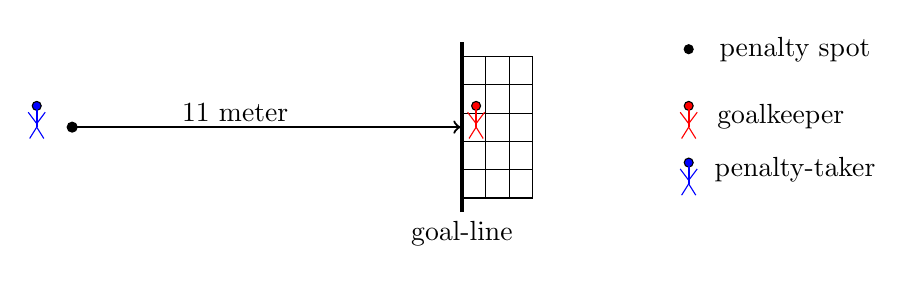
\begin{tikzpicture} [scale=0.9]
%\draw (0,1.3) node[below] {$B$} --
%(3,1.3) node[below] {$C$};
%\fbox{1.Bestimmung einer Startl\"{o}sung} \\
%\fbox{2.Aktualisierung der Werte} \\
%\fbox{3.Terminierung des Algorithmus}

\draw[fill=black](0,1.0)circle(2pt); 
\draw[-,very thick] (5.5,-0.2)--(5.5,2.2);
\draw[-,thin] (5.5,2) --(6.5,2);
\draw[-,thin] (5.5,0) --(6.5,0);
\draw[-,thin] (6.5,0) --(6.5,2);
\draw[->,thick] (0.05,1)--(5.48,1);
\draw[-,very thin] (5.833,2) --(5.833,0);
\draw[-,very thin] (6.166,0) --(6.166,2);
\draw[-,very thin] (5.5,0.4) --(6.5,0.4);
\draw[-,very thin] (5.5,0.8) --(6.5,0.8);
\draw[-,very thin] (5.5,1.2) --(6.5,1.2);
\draw[-,very thin] (5.5,1.6) --(6.5,1.6);
%\draw[-, very thin] (5.5,0) --(6.5,0);
\draw node[black] at (2.3,1.2) {11 meter};
\draw node[black] at (5.5,-0.5) {goal-line};
\draw[fill=black](8.7,2.1)circle(1.8pt);
\draw node[black] at (10.2,2.1) {penalty spot};


%%%goalkeeper
\draw[fill=red](8.7,1.3)circle(1.8pt); 
\draw[-,red,thick](8.7,1.3)--(8.7,1);
\draw[-,red](8.7,1.05)--(8.58,1.21);
\draw[-,red](8.7,1.05)--(8.82,1.21);
\draw[-,red](8.7,1)--(8.6,0.84);
\draw[-,red](8.7,1)--(8.8,0.84);
\draw node[black] at (10,1.15) {goalkeeper};


\draw[fill=red](5.7,1.3)circle(1.8pt); 
\draw[-,red,thick](5.7,1.3)--(5.7,1);
\draw[-,red](5.7,1.05)--(5.58,1.21);
\draw[-,red](5.7,1.05)--(5.82,1.21);
\draw[-,red](5.7,1)--(5.6,0.84);
\draw[-,red](5.7,1)--(5.8,0.84);

%%%penalty taker
\draw[fill=blue](-0.5,1.3)circle(1.8pt); 
\draw[-,blue,thick](-0.5,1.3)--(-0.5,1);
\draw[-,blue](-0.5,1.05)--(-0.62,1.21);
\draw[-,blue](-0.5,1.05)--(-0.38,1.21);
\draw[-,blue](-0.5,1)--(-0.6,0.84);
\draw[-,blue](-0.5,1)--(-0.4,0.84);


\draw[fill=blue](8.7,0.5)circle(1.8pt); 
\draw[-,blue,thick](8.7,0.5)--(8.7,0.2);
\draw[-,blue](8.7,0.25)--(8.58,0.41);
\draw[-,blue](8.7,0.25)--(8.82,0.41);
\draw[-,blue](8.7,0.2)--(8.6,0.04);
\draw[-,blue](8.7,0.2)--(8.8,0.04);
\draw node[black] at (10.2,0.4) {penalty-taker};

%\draw [->,very thick] (-3.66,2.44) -- (3.66,2.44);
%\draw [-,very thick] (-3.66,0) -- (-3.66,2.44);
%\draw [-,very thick] (3.66,2.44) -- (3.66,0);
%\draw [-,thick] (-3.66,1.62) -- (3.66,1.62);
%\draw [-,thick] (-3.66,1.22) -- (3.66,1.22);
%\draw [-,thick] (-1.22,2.44) -- (-1.22,0);
%\draw [-,thick] (1.22,2.44) -- (1.22,0);
%\draw [-,thin] (-3.7,0) -- (3.7,0);

\end{tikzpicture}
\label{fig:dtmc2}
\end{center}
\end{figure}

%\begin{figure}[ht]
%\begin{center}
%\caption{Football Goal}
%\begin{tikzpicture}
%\draw (0,1.3) node[below] {$B$} --
%(3,1.3) node[below] {$C$};
%\fbox{1.Bestimmung einer Startl\"{o}sung} \\
%\fbox{2.Aktualisierung der Werte} \\
%\fbox{3.Terminierung des Algorithmus}

%\draw [-,very thick] (-3.66,2.44) -- (3.66,2.44);
%\draw [-,very thick] (-3.66,0) -- (-3.66,2.44);
%\draw [-,very thick] (3.66,2.44) -- (3.66,0);
%\draw [-,thick] (-3.66,1.62) -- (3.66,1.62);
%\draw [-,thick] (-3.66,1.22) -- (3.66,1.22);
%\draw [-,thick] (-1.22,2.44) -- (-1.22,0);
%\draw [-,thick] (1.22,2.44) -- (1.22,0);
%\draw [-,thin] (-3.7,0) -- (3.7,0);

%\end{tikzpicture}
%\label{fig:dtmc2}
%\end{center}
%\end{figure}

\vspace{-0.5cm}

In this thesis, we handle two main tasks. The first task is to collect and prepare suitable data of penalties. Since high quality data is difficult to get and can be expensive, we decide to create our own collection of penalties. For that, we first investigate the current literature and try to find potential variables influencing the shot performance and behavior. In the next step, we collect penalty data using different sources, especially regarding the potential variables identified by the literature review and some self-identified variables. Both processes, we describe in more detail in the next section. \\
%
%
The second task is to estimate a discrete choice model of the penalty-taker's behavior. For a goalkeeper to save a penalty, it is crucial to know, where the penalty-taker wants to shoot the ball. Since the penalty-taker has a lot of different possibilities to shoot the ball, predicting the correct direction can get a difficult task. In our model, we assume that the penalty-taker has six different alternatives to shoot on the goal, which we show in figure 2. We divide the goal one time horizontally into flat and high shots. Furthermore, we divide the goal two times vertically, so the penalty-taker can decide to shoot to his left, to the center or to his right. In this thesis, regarding the penalty shot directions and the movements of the goalkeeper, we are always considering the point of view of the penalty-taker. The possibility of shooting beside the goal or just hitting the goalpost or the crossbar are included in the alternatives. For example, shots like the points x1 and x2 belong to the alternative TL. These shots are "missed". Shots are also missed, if the ball hits the goalpoast/crossbar and afterwards bounces from the goalkeeper into the goal. Furthermore, figure 2 shows the measures of a goal. From the ground to the crossbar the goal measures 2.44 m and between the goalposts it measures 7.32 m.


 \begin{figure}[h]
 \begin{center}
 \caption{Soccer goal with the considered alternatives}
 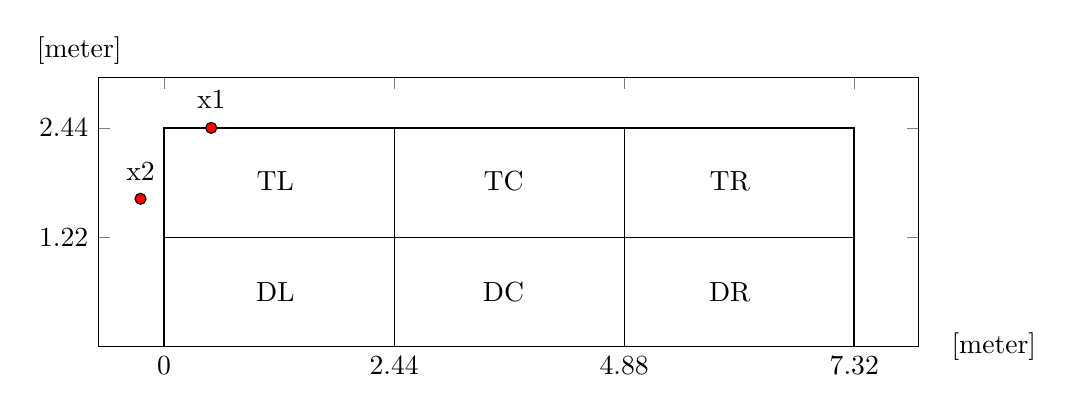
\begin{tikzpicture}
\begin{axis}
[%axis x line=center,
  %axis y line=center,
    width=12cm,
  height=5cm,
  xtick={0,2.44,4.88,7.32},
  ytick={1.22,2.44},
  xlabel style={right},
  ylabel style={above},
  clip=false,
  xmin=-0.70, xmax=8, ymin=0, ymax=3]
  \draw [black, thick] (axis cs:0,0)-- (axis cs:0,2.44) -- (axis cs: 7.32,2.44) -- (axis cs:7.32,0);
 %  \draw [black, thin] (axis cs:0,0.81)-- (axis cs:7.32,0.81);
  \draw [black, thin] (axis cs:0,1.22)-- (axis cs:7.32,1.22);
  \draw [black, thin] (axis cs:2.44,0)-- (axis cs:2.44,2.44);
  \draw [black, thin] (axis cs:4.88,0)-- (axis cs:4.88,2.44);
  
   \draw[fill=red](axis cs:0.5,2.44)circle(2pt); 
   \draw node[black] at (axis cs: 0.5,2.75) {x1};
  \draw[fill=red](axis cs:-0.25,1.65)circle(2pt); 
   \draw node[black] at (axis cs: -0.25,1.95) {x2};
  
%  \def\RADIUS{2.84cm} 
%  \coordinate[label=left:$O$] (O) at (0,0);
%   \coordinate[label=below:$D$] (D) at (-\RADIUS,0);
%Halbkreis zeichnen
%\draw[name path=HALFCIRCLE] ([shift=(180:\RADIUS)]O) arc (180:0:\RADIUS) to (D);
   
  \draw node[black] at (axis cs: 1.18,1.85) {TL};
  \draw node[black] at (axis cs: 3.6,1.85) {TC};
  \draw node[black] at (axis cs: 6,1.85) {TR};
  \draw node[black] at (axis cs: 1.18,0.61) {DL};
  \draw node[black] at (axis cs: 3.6,0.61) {DC};
  \draw node[black] at (axis cs: 6,0.61) {DR};
%   \draw[fill=green](axis cs:78,1.15)circle(2pt); 
   \draw node[black] at (axis cs: -0.9,3.3) {\normalsize [meter]};
  \draw node[black] at (axis cs: 8.8,0) {\normalsize [meter]};
%  \draw node[black] at (axis cs: 0.3,1.8) {\normalsize $EBO^{obj}$ [in u]};
  %\draw [black, thick] (axis cs:0.05,-0.3)--(axis cs:0.05,0.3);
    %\draw [black, thick] (axis cs:0.15,-0.3)--(axis cs:0.15,0.3);
     %\draw [black, thick] (axis cs:0.25,-0.3)--(axis cs:0.25,0.3);
      %\draw [black, thick] (axis cs:0.35,-0.3)--(axis cs:0.35,0.3);
\end{axis}
\end{tikzpicture}
\end{center}
\end{figure}

\vspace{-1cm}

\section{Data Collection, Preparation and Analysis}
In the following section, we present our collected data and show how we find potential interesting variables, from which sources we compile the data and how we prepare it to ensure high quality. Furthermore, we shortly analyze the data regarding the most important statistics. 

\subsection{Literature Review}
The literature review shall give an overview and help to detect interesting and potential variables of predicting the behavior of the penalty-taker. 
%The penalty kick as we know was introduced in 1902. Since 1906 the goalkeeper has to stay on or behind the goalline at the moment of the shot and can not move forward.[1]https://www.fussballtrainer.de/fussballgeschichte/geschichte-der-fussballregeln.html From 1929 to 1997, the goalkeeper is restricted more and needs to stay on the goalline and was not allowed to move on his goalline. After the change in 1997, the goalkeeper can move laterally on his goalline, which makes the penalty more complex [2] (Dalton,Guillon, Naroo 2015). The last change in rule was in June 2019. The goalkeeper just needs to stay with at least one foot on the or behind the goalline, the other foot can be placed before. In this thesis we only consider penalties after 1997. \\
A possible partition of the investigations of penalty kicks in the literature is just considering in-match penalties (see e.g. Horn et al. (2020, p.139-155)) and penalty shootouts (see e.g. Hughes \& Wells (2002, p.55-72), Krumer (2020, 101578)). In his research, Krumer (2020,101578) ascertains that the teams playing in a higher league than their opponent have a greater chance of winning the penalty shootout. Inspired from this research, in this thesis, we consider being the favored team (respectively the underdog) as potential influencing variable for shooting a penalty. \\  
Buzzacchi \& Pedrini (2014, p.1067-1080) state that the behavior of the penalty-takers is rational and, under specific circumstances, it can not always be recognized.  Furthermore, they mention that high quality players are easier to predict since they are more often shooting  to their preferred direction/their natural side. The natural side is for a right-footed penalty-taker the left side of the goal, and for a left-footed penalty-taker the right side of the goal. Regarding the high quality players, Baumann et al. (2011, p.81-105) present the same result, too. In this thesis, we especially consider high quality players and regard the footedness (i.e. strong foot of player) of the penalty-taker. \\
%
%Eventuell unnützer Part, keine Conclusion for die Arbeit
%The anticipation of the shot direction is in literature reviewed under a lot of different factors. On the one hand the anticipation of the goalkeeper to predict the shot direction is investigated a lot. On the other hand the anticipation of the penalty-taker regarding the movement of the goalkeeper is of interest, too. Two main factors for goalkeepers to predict the shot direction are the gaze (e.g. Kim and Lee 2006) and the body (e.g. Diaz and Fajen 2006). Hereby the body can be seperated into several different body parts (like the positioning of the non-kicking foot (Li et al 2015), which should help to anticipate the shot direction. A good general overview about the influence of specific body parts is given by (Lees et al 2010). \\
% new part
A time-depending performance analysis of penalty kicks is made by Almeida et al. (2016, p.508-522). They divide the match into three thirds of half an hour and could find differences in performance regarding these parts. We conclude that the point in time can be decisive and a variable of interest. \\
With increasing minutes played, the players also get more fatigue. The fatigue as potential influencing factor on the performance is analyzed by Jordet et al. (2007, p.121-129). Overall, fatigue has a small influence on the performance. More interesting is the detection of these authors that stress, indicated by the importance of the match, has a negative influence on the performance of the penalty-taker. Consequently, we will test the importance of a match as a potential influencing variable. \\
%
%The success of a penalty depends mostly on the two variables angle at which the shot is kicked and the velocity of the ball. (Leela and Cosmoring 2009). These authors conclude that if the ball is kicked in the right measure of both, it almost always find it way into the goal, independent of the goalkeepers action.
For maximizing success, the penalty-taker should shoot the ball with a high accuracy. The accuracy is already influenced by the pure presence of a goalkeeper (see Navarro et al. (2011, p.921-929)). The same counts, when the goalkeeper is moving (see Wood \& Wilson (2010, p.937-946)). Based on these assumptions, Lidor et al. (2012, p.375-389) show the occurrence of misleading strategies (e.g. standing off-center), which help the goalkeeper to influence the penalty-taker to shoot in the goalkeeper's wanted direction. \\
\\ 
Already, Chiappori et al. (2002, p.1138-1151) mention that the behavior of the penalty-taker probably depends on the behavior of the goalkeeper. This is also valid, when the penalty-taker is using a so-called keeper-dependent strategy \mbox{(see Noel et al. 2015, p.1-10)}. Using this strategy, the penalty-taker reacts to the movements of the goalkeeper, which potentially lead to a change of the previous desired shot direction. Overall, we conclude that the movement and position of the goalkeeper are possible variables influencing the penalty-taker. Thus, we include these in our data collection.\\
A further research regarding the goalkeeper was done by M\"uller et al. \mbox{(2018, p.128-134).} They show that a goalkeeper with a high reputation influences the shot performance of a penalty-taker negatively and is observed taller than a low reputation goalkeeper.
Further potential influencing factors of the performance of a penalty kick (in penalty shootouts) are analyzed by Noel et al. (2014, p.51-62). They investigate for example the jersey color and the experience. Even though not all factors are relevant for success, we still consider some of them as potential variable for predicting the shot direction. \\
Even if most researchers mentioned rather consider the performance of the penalty kick, the mentioned variables possibly influence the shot direction, too. Overall, we are able to derive several ideas from the literature regarding potential variables.
%- natural side
%- keeper has no time to react
%The ball needs around 0.3 seconds from the penalty spot to the goal line. (Palacios-Huerta 2003). ... unwichtig
%- keeper stands mostly in the middle
%- bias shot to the rihgt?
%- kürzen unwichtige sachen raus wie ballgeschwindigkeit, zusammenfassen von high quality spielern; game theory kacke raus
%- in shootout lead or not affects ... Jordet


\subsection{Collecting and Preparing of Data and Variables}

For collecting the data, we use a lot of different sources. This enables a high quality, because the information of the different sources could be compared and consequently checked for correctness. A list of all used sources can be found in the appendix.  \\
The database comprises 2358 penalties. The following table gives a short overview of the different competitions and the years/seasons which can be found in our database.

\vspace{+0.3cm}

 \begin{table}[h]
\caption{Competitions in database}
\centering
\begin{tabular}{ c | c }
    $competition$ & $year/season$   \\
   \hline

German "Bundesliga"  & 2018/19, 2019/20, 2020/21 \\

"DFB-Pokal"  & 2018/19, 2019/20, 2020/21 \\

World Cup & 2006, 2010, 2014, 2018 \\   
   
European Championship  & 2008, 2012, 2016, 2021 \\

 \end{tabular}
 \end{table}
 
 \vspace{+0.3cm}
 

The database contains the penalties (in-match and shootout) of all German "Bundesliga" clubs of the seasons mentioned, including the competitions "DFB-Pokal", "Europa League" and "Champions League". Furthermore, we collect the penalties of the opponents of the Bundesliga clubs in a penalty shootout, too. Moreover, the database contains all penalties (in-match and shootout) of the World Cup and European Championship of the last 15 years. Last but not least, almost all penalties of several (high quality) players e.g. Ronaldo and Messi we include in the database. The full list of all players, which we investigate, can be found in the appendix. The choice of the single players is rather random and hardly under some specific conditions. We try to find both very good penalty-takers and rather bad penalty-takers. The main factors are to investigate famous players, from which almost all penalties can be considered. Moreover, regarding the choice of the penalty-taker, we try to balance between right-footed and left-footed players and between the different player positions.  \\
The data for the single penalties we mainly derive from "www.transfermarkt.de". On this website there is for every player a detailed list of all shot penalties. Each penalty is linked to the match, where the penalty was shot and from there we derive the main data like minute, scoreline, goalkeeper etcetera. The website "www.kicker.de" we use to check and confirm the presented information. The shot directions, we mainly get by video analyzing via the platforms "YouTube.com" and "dailymotion.com", where the highlights of the single matches containing the penalties are uploaded. There are a lot of different uploaders, the most used are: "DAZN", "Bild" and the official channels of the clubs and competitions. This kind of data is free available, nevertheless, it is licensed, and so we can guarantee to have the correct data. For almost all penalties, we use a video analysis, which mostly shows the entire penalty from at least two different camera perspectives. In just a few cases, we estimate the shot direction by using pictures and reports e.g. from "www.kicker.de".  \\
For that few cases, we have no information concerning the movement and the position of the goalkeeper during the run-up of the penalty-taker, which is needed for several variables. Furthermore, we do the video analyze manually by a human and not by a computer. Considering the shot direction and the position of the goalkeeper, we are limited and just do estimates. Consequently, we can not guarantee to have perfectly correct data. Nevertheless, we are convinced to have high quality and suited data.
%

We derive the data manually, which should not but can lead to small errors, which simultaneously is a limitation of our model estimation. We periodically check the data for correctness, considering typing errors etcetera. Moreover, we try to avoid errors by preparing the data using the software Excel and RStudio. In the following, we present some potential errors, which we fixed: 

\begin{tabular}[t]{lr} 
-- check age, e.g. age not under 16 or over 45 \\ 
-- check height of goalkeeper, e.g. not under 1.7 m and not over 2.2 m \\ 
-- check same goalkeeper has always same height  \\
-- check same player/goalkeeper always gets the same name \\
-- check no redundant penalty \\
-- check dates, e.g. no penalty before 2000 or after 2021 \\
%-- check logical correct score by regarding scoreline, Home/Away and "Lead-Deficit" \\
-- check actual result \\
%-- check whether all penalties of an individual player are in database \\
-- check whether number of goals/fails of an individual player is correct. \\
\end{tabular}

\vspace{+0.5cm}
Furthermore, we video analyzed all penalties at least three times, always on a different day, to minimize errors especially regarding the shot direction.  \\
Considering our identified variables, we always have at least 90 penalties, including the single values of each variable. This should help to avoid overfitting.  The full list of all variables, shortly explained, we present in the tables 11-16 in the appendix. \\

%-used RStudio to check quality like goalkeeper have always the same height .... 
%-- check logical correct score by regarding scoreline, Home/Away and "Lead-Deficit" \\
%- score is logical correct in for Home and Away teams ... looking at ABA which kind of mistake we proove  \\
%- score with one goal difference gets a + or - 1 and not a something wrong \\
%- no penalty twice in the data set \\
%- checking dates, whether there is no potential wrong date, like penalty in future, or penalty of the EM in a year, where no EM was
%- checking whether we found all penalties of the individual players are found \\
%- checking whether there is no incidentally marking a goal as a non-goal or a non-goal as a goal \\
%- checking age \\
%Later: For the well-placed shots weniger Elfmeter; slipped away shots excluded.
%- first how we get the data, naming all sources like kicker, www.sport.de, transfermarkt.de and so on. 
%- used videos on youtube and daily motion ... published by dazn, bild.de ,sportbild and so on ... and fans in the stadion which have filmed the penalt ... so used at usually at least two differenct camera perspectives 
%- data is very costly

%- explaining the variables \\
%- how data is gained and prepared \\
%- explaining what is considered \\


%In the following we shortly present some of the identified possible factors for determining the shot direction.

\vspace{-0.7cm}

\subsection{Data Analysis}

In the following section, we present a short general analysis of the data and then focus on analyzing the success rate of the penalties. We especially consider the single alternatives mentioned in the problem description. We refrain from analyzing each variable in detail, since we want to avoid making an analysis of an irrelevant variable. \\
The database consists of 2358 penalties shot by 485 different players. These penalty-takers are in average rounded 27 years old, whereby the youngest player is 16 and the oldest is 40. All in all, we have 1421 penalties shot by a striker, 698 penalties shot by a midfielder, 237 penalties shot by a defender and two penalties shot by a goalkeeper. We consider 1834 in-match penalties and 524 penalties shot in a penalty shootout. \\
The goalkeeper stands in 92.2\% of the penalties in the center of the goal. Standing at the left (3.42\%) or right (4.36\%) side has almost the same probability and overall, it is relative unusual. In rounded one third of the cases (33.7 \%) the goalkeeper is moving during the run-up of the penalty-taker. The average height of the goalkeepers amounts to a rounded 1.90 m, whereby the range is between 1.76 m and 2.03 m. \\
The penalties result in 1873 cases to a goal (79.43 \%), 351 times the ball is saved by the goalkeeper (14.89 \%) and 134 times the penalty-taker misses the goal (5.68 \%). 

\vspace{0.1cm}

\begin{figure}[ht]
\begin{center}
\caption{Probabilities of alternatives chosen in database}
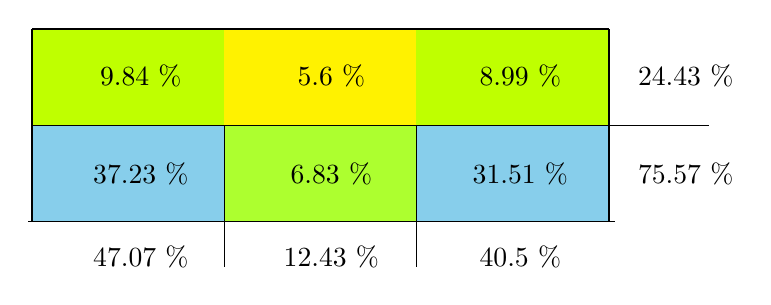
\begin{tikzpicture}
%\draw (0,1.3) node[below] {$B$} --
%(3,1.3) node[below] {$C$};
%\fbox{1.Bestimmung einer Startl\"{o}sung} \\
%\fbox{2.Aktualisierung der Werte} \\
%\fbox{3.Terminierung des Algorithmus}

\draw [-,very thick] (0,2.44) -- (7.32,2.44);
\draw [-,very thick] (0,0) -- (0,2.44);
\draw [-,very thick] (7.32,2.44) -- (7.32,0);
%\draw [-,thick] (-3.66,1.62) -- (3.66,1.62);
\draw [-,thick] (0,1.22) -- (7.32,1.22);
\draw [-,thin] (-0.05,0) -- (7.4,0);
\draw [-,thin] (2.44,0) -- (2.44,-0.58);
\draw [-,thin] (4.88,0) -- (4.88,-0.58);
\draw [-,thin] (7.32,1.22) -- (8.6,1.22);

  \path[fill=SkyBlue,draw=black]
        (0,0)
        -- (0,1.22)
        -- (2.44,1.22)
        -- (2.44,0);   
        
       \path[fill=SkyBlue,draw=black]
        (4.88,0)
        -- (4.88,1.22)
        -- (7.32,1.22)
        -- (7.32,0); 
        
        
            \path[fill=GreenYellow,draw=black]
        (2.44,0)
        -- (2.44,1.22)
        -- (4.88,1.22)
        -- (4.88,0); 
        
            \path[fill=lime,draw=black]
        (0,1.22)
        -- (0,2.44)
        -- (2.44,2.44)
        -- (2.44,1.22); 
        
            \path[fill=yellow,draw=black]
        (2.44,1.22)
        -- (4.88,1.22)
        -- (4.88,2.44)
        -- ( 2.44,2.44); 
        
      \path[fill=lime,draw=black]
        (4.88,1.22)
        -- (7.32,1.22)
        -- (7.32,2.44)
        -- (4.88,2.44); 
        
          \draw node[black] at (1.38,1.85) {9.84 \%};
  \draw node[black] at (3.8,1.85) {5.6 \%};
  \draw node[black] at (6.2,1.85) {8.99 \%};
  \draw node[black] at (1.38,0.61) {37.23 \%};
  \draw node[black] at (3.8,0.61) {6.83 \%};
  \draw node[black] at (6.2,0.61) {31.51 \%}; 
  \draw node[black] at (1.38,-0.45) {47.07 \%};
  \draw node[black] at (3.8,-0.45) {12.43 \%};
  \draw node[black] at (6.2,-0.45) {40.5 \%};
  \draw node[black] at (8.3,1.85) {24.43 \%};
  \draw node[black] at (8.3,0.61) {75.57 \%};

\end{tikzpicture}
\label{fig:dtmc2}
\end{center}
\end{figure}

\vspace{-0.3cm}

In figure 3, we show the probabilities of the penalties shot to the different alternatives. The most penalties are shots in the down corners, whereby the ball has shot more often to the down left corner (37.23 \%). The next most probable chosen alternatives are the top corners, whereby again the left corner is more often chosen than the right corner. Overall, the penalty-takers shot the ball in a rounded three-quarters rather flat to the goal. 

\vspace{+0.5cm}

\begin{figure}[ht]
\begin{center}
\caption{Probability of goal,save and miss of each alternative}
\begin{tikzpicture}[scale = 0.96]
\begin{axis}[
width=14cm, height =7cm,
ybar,enlargelimits=0.15,
symbolic x coords={TL,TC,TR,DL,DC,DR},xtick={TL,TC,TR,DL,DC,DR},
legend style={
  at={(current bounding box.south-|current axis.south)},
  anchor=north,
  legend columns=-1
},
]


\addplot +[fill=blue] coordinates 
{(TL,81.46) (TC,80.3) (TR,81.13)(DL,79.15) (DC,75.78) (DR,79.27)};
\addplot+[fill=red] coordinates
{(TL,6.46) (TC,3.79) (TR,3.3)(DL,16.86) (DC,24.22) (DR,18.44)};
\addplot +[fill=yellow] coordinates
{(TL,12.07) (TC,15.9) (TR,15.57)(DL,3.99) (DC,) (DR,2.23)};

\node[blue]  at(-10,835){81.46 $\%$};
\node[rotate=90, red]   at(0,165){6.46 $\%$};
\node[rotate=90, black] at(22,241){12.07 $\%$};

\node[blue]  at(90,822){80.3 $\%$};
\node[rotate=90, red]   at(100,141){3.79 $\%$};
\node[rotate=90, black] at(122,267){15.9 $\%$};

\node[blue]  at(190,825){81.13 $\%$};
\node[rotate=90, red]   at(200,118){3.3 $\%$};
\node[rotate=90, black] at(222,277){15.57 $\%$};

\node[blue]  at(290,812){79.15 $\%$};
\node[rotate=90, red]   at(300,292){16.86 $\%$};
\node[rotate=90, black] at(322,140){3.99 $\%$};

\node[blue]  at(390,780){75.78 $\%$};
\node[rotate=90, red]   at(400,367){24.22 $\%$};
\node[rotate=90, black] at(422,40){0 $\%$};

\node[blue]  at(490,815){79.27 $\%$};
\node[rotate=90, red]   at(500,307){18.44 $\%$};
\node[rotate=90, black] at(522,135){2.23 $\%$};

\legend{Goals,Saves,Misses} 


\end{axis}
\end{tikzpicture} 
\end{center}
\end{figure}

\vspace{-0.3cm}

Figure 4 shows the single percentages of goals, saves and misses regarding the single alternatives. In all cases, shooting a goal is the most probable. The highest probability of shooting a goal is given by shooting the ball to one of the top corners, since these corners the goalkeeper can not cover completely. The probabilities amount to 81.46\% for the left top corner and 81.13\% for the right top corner. \\
Another clear observation is that the shots to the top of the goal have a higher chance of being missed than being saved. Reasons are that high shots can be shoot over and beside the goal, but therefor, the goalkeeper has a relative small coverage to save those. The opposite is valid for flat shots, where the save rate is clearly higher than the miss rate. Considering these shots, the goalkeeper has a relative high coverage. The ball can not be shoot under the goal, thus, flat shots can only be missed by shooting beside the goal. That is why DC has a miss probability of 0\%, since it is not possible. However, DC has the highest probability of being saved. \\
%
In the literature review, we mentioned a "natural side" of the penalty-taker, depending on their strong foot. In the following, we analyze this phenomenon by considering left-footed and right-footed penalty-takers. We display a comparison in figure 5. In our database, we have 579 penalties shot by a left-footed player and 1779 penalties shot by a right-footed player.

\begin{figure}[ht]
\begin{center}
\caption{Comparison left-footed and right-footed penalty-takers}
\begin{minipage}[t]{0.45\linewidth}
  \centering
\begin{tikzpicture}[scale=0.95,baseline=(current axis.south)]
%\draw (0,1.3) node[below] {$B$} --
%(3,1.3) node[below] {$C$};
%\fbox{1.Bestimmung einer Startl\"{o}sung} \\
%\fbox{2.Aktualisierung der Werte} \\
%\fbox{3.Terminierung des Algorithmus}
\draw [-,very thick] (0,2.44) -- (7.32,2.44);
\draw [-,very thick] (0,0) -- (0,2.44);
\draw [-,very thick] (7.32,2.44) -- (7.32,0);
%\draw [-,thick] (-3.66,1.62) -- (3.66,1.62);
\draw [-,thick] (0,1.22) -- (7.32,1.22);
\draw [-,thin] (-0.05,0) -- (7.4,0);

   \path[fill=Cyan,draw=black]
        (0,0)
        -- (0,1.22)
        -- (2.44,1.22)
        -- (2.44,0);   
        
       \path[fill=VioletRed,draw=black]
        (4.88,0)
        -- (4.88,1.22)
        -- (7.32,1.22)
        -- (7.32,0); 
        
        
            \path[fill=Yellow,draw=black]
        (2.44,0)
        -- (2.44,1.22)
        -- (4.88,1.22)
        -- (4.88,0); 
        
            \path[fill=SkyBlue,draw=black]
        (0,1.22)
        -- (0,2.44)
        -- (2.44,2.44)
        -- (2.44,1.22); 
        
            \path[fill=GreenYellow,draw=black]
        (2.44,1.22)
        -- (4.88,1.22)
        -- (4.88,2.44)
        -- ( 2.44,2.44); 
        
      \path[fill=Lavender,draw=black]
        (4.88,1.22)
        -- (7.32,1.22)
        -- (7.32,2.44)
        -- (4.88,2.44); 
        
          \draw node[black] at (1.38,1.85) {7.25 \%};
  \draw node[black] at (3.8,1.85) {3.45 \%};
  \draw node[black] at (6.2,1.85) {14.33 \%};
  \draw node[black] at (1.38,0.61) {29.88 \%};
  \draw node[black] at (3.8,0.61) {6.75 \%};
  \draw node[black] at (6.2,0.61) {38.34 \%};
    \draw node[black] at (1.38,-0.45) {37.13 \%};
  \draw node[black] at (3.8,-0.45) {10.2 \%};
  \draw node[black] at (6.2,-0.45) {52.67 \%};
  
  \draw node[black] at (3.9,2.7) {left-footed}; 
\end{tikzpicture}
\end{minipage}
\hfill
\begin{minipage}[t]{0.45 \linewidth}
\centering
\begin{tikzpicture}[scale=0.95,baseline=(current axis.south)]
%\draw (0,1.3) node[below] {$B$} --
%(3,1.3) node[below] {$C$};
%\fbox{1.Bestimmung einer Startl\"{o}sung} \\
%\fbox{2.Aktualisierung der Werte} \\
%\fbox{3.Terminierung des Algorithmus}

\draw [-,very thick] (0,2.44) -- (7.32,2.44);
\draw [-,very thick] (0,0) -- (0,2.44);
\draw [-,very thick] (7.32,2.44) -- (7.32,0);
%\draw [-,thick] (-3.66,1.62) -- (3.66,1.62);
\draw [-,thick] (0,1.22) -- (7.32,1.22);
\draw [-,thin] (-0.05,0) -- (7.4,0);


  \path[fill=Cyan,draw=black]
        (0,0)
        -- (0,1.22)
        -- (2.44,1.22)
        -- (2.44,0);   
        
       \path[fill=VioletRed,draw=black]
        (4.88,0)
        -- (4.88,1.22)
        -- (7.32,1.22)
        -- (7.32,0); 
        
        
            \path[fill=Yellow,draw=black]
        (2.44,0)
        -- (2.44,1.22)
        -- (4.88,1.22)
        -- (4.88,0); 
        
            \path[fill=SkyBlue,draw=black]
        (0,1.22)
        -- (0,2.44)
        -- (2.44,2.44)
        -- (2.44,1.22); 
        
            \path[fill=GreenYellow,draw=black]
        (2.44,1.22)
        -- (4.88,1.22)
        -- (4.88,2.44)
        -- ( 2.44,2.44); 
        
      \path[fill=Lavender,draw=black]
        (4.88,1.22)
        -- (7.32,1.22)
        -- (7.32,2.44)
        -- (4.88,2.44); 
        
          \draw node[black] at (1.38,1.85) {10.68 \%};
  \draw node[black] at (3.8,1.85) {6.3 \%};
  \draw node[black] at (6.2,1.85) {7.25 \%};
  \draw node[black] at (1.38,0.61) {39.63 \%};
  \draw node[black] at (3.8,0.61) {6.86 \%};
  \draw node[black] at (6.2,0.61) {29.28 \%};
  \draw node[black] at (1.38,-0.45) {50.31 \%};
  \draw node[black] at (3.8,-0.45) {13.16 \%};
  \draw node[black] at (6.2,-0.45) {36.53 \%};
  
  \draw node[black] at (3.9,2.7) {right-footed}; 


\end{tikzpicture}
\end{minipage}
\end{center}
\end{figure}

\vspace{-0.3cm}

Regarding our database, we are able to confirm the phenomenon. It is clearly to observe that left-footed players more likely shoot to their right side. Vice versa, we can see that right-footed players more likely shoot to their left side. Both shoot over the half of their penalties to their "natural side" \\
Whether the ball has shot rather flat or rather high is not affected by this phenomena. Equally to the general analysis from figure 3, we can ascertain that the shots are in circa three-quarter of the cases rather flat. %The likelihood of shooting to the alternative "DC" is for both almost the same.  \\
Interesting to observe is that, given a left-footed penalty-taker has shot to the top of the goal, shooting to their natural side is not only the most probable alternative, it is more probable than the other two alternatives together \mbox{(14.33\% $>$ 10.7\%).} Comparatively, for right-footed players shooting to the top, the natural side is admittedly the most probable, but not more likely than the other two alternatives together \mbox{(10.68\% $<$ 13.55\%).}\\

%\begin{figure}[ht]
%\caption{distribution of chosen alternatives considering "well-placed" shots}
%\begin{minipage}{0.68\textwidth}
%  \centering
%\begin{tikzpicture}[scale=1.4]
%\pie[radius=2,after number= , sum=auto, color={RubineRed, Melon, Goldenrod, RoyalBlue, Cyan, SeaGreen, OliveGreen, Yellow, Orchid, RedViolet}]
%{124/TLP , 108/TLNP , 132/TC , 99/TRNP , 113/TRP ,  283/DRP , 452/DRNP , 161/DC, 454/DLNP , 418/DLP}
%\end{tikzpicture}
%\caption{Distribution "well-placed" shots}
%\label{fig:Distribution of chosen alternatives considering "well-placed" shots}
%\end{minipage}%
%\hfill
%\begin{minipage}{0.32\textwidth}
 % \centering
%\begin{tabular}{ c | c }
%    $Alternative$ & $Probability$   \\
%   \hline%
%
%TLP  & 5.29 \%  \\

%TLNP & 4.61 \% \\   
  
%TC & 5.63 \%  \\  

%TRNP  & 4.22 \% \\

%TRP  & 4.82 \%  \\

%DLP & 17.83 \%  \\

%DLNP & 19.37 \%  \\   
  
%DLC & 6.87 \%   \\  

%DRNP   & 19.28 \%  \\

%DRP  & 12.07 \%  \\


 %\end{tabular}
 %\captionof{table}{"Well-placed" shots}
 %\label{tab:my-label}
 %\end{minipage}
%\end{figure}


\section{Model Estimation and Results}

\subsection{Mathematical Model}

%\begin{figure}[ht]
%\begin{center}
%\caption{Greedy algorithm for system-approach}
%\begin{tikzpicture}
%\draw (0,1.3) node[below] {$B$} --
%(3,1.3) node[below] {$C$};
%\fbox{1.Bestimmung einer Startl\"{o}sung} \\
%\fbox{2.Aktualisierung der Werte} \\
%\fbox{3.Terminierung des Algorithmus}
%\node[draw,text width=5.5cm] at (1.5,2){ 1. Determine $EBO^{obj}$, Set $S_i = 0$ for all %i$\in$I};
%\node[draw,text width=5.5cm] at (1.5,0.5){ 2. Determine $S_i$ to increase};
%\node[draw,text width=5.5cm] at (1.5,-1){ 3. Update C(S) and EBO(S)};
%\draw [->,very thick] (1.5,1.41) -- (1.5,0.82);
%\draw [->,very thick] (1.5,0.18) -- (1.5,-0.68);
%\node[draw,text width=4cm] at (1.5,-2){ EBO(S) $<EBO^{obj}$ ?};
%\draw [-,very thick] (1.5,-1.32) -- (1.5,-1.61);
%\node[draw,text width=0.9cm] at (0,-3.2){No!};
%\node[draw,text width=0.9cm] at (3,-3.2){ Yes!};
%\node[draw,text width=1.5cm] at (3,-4.2){solution};
%\draw [-,very thick] (-0.572,-3.2) -- (-3,-3.2)-- (-3,0.5);
%\draw [->,very thick] (-3,0.5) -- (-1.4,0.5);
%\draw [->,very thick] (1.5,-2.38) -- (0.5,-2.95);
%\draw [->,very thick] (1.5,-2.38) -- (2.5,-2.96);
%\draw [->,very thick] (3,-3.49) -- (3,-3.90);

%\end{tikzpicture}
%\label{fig:dtmc2}
%\end{center}
%\end{figure}

In the following section, we present the model. The assumptions and the model are based on the general model for discrete choice models made by Koppelman \& Bhat (2006, p.14-60). We will consider a utility-based model, whereby we assume that the decision maker chooses (C) the alternative which is giving him the highest utility U. The choice is unique, since the utility values differ clearly among the alternatives.

\vspace{-1.5cm}
 
\begin{center}
\begin{align}
 C = \{ i | U_{it} = max(U_{it}) \} \\
 U_{it} = V_{it} + \epsilon_{it} \label{eq:test2}
\end{align}
\end{center}

\vspace{-0.5cm}

The utility $U_{it}$, we calculate for each single alternative i given the decision maker t. It is comprised by two parts. The first part is the utility estimated by the analyst based on his observations. The second part is the utility, which is not observable and so not measurable for the analyst. This part is known as error term. It is used to include all factors into the model which otherwise would not be in the model. \\
%
The observable part of the utility is calculated by the addition of three parts:

\vspace{-1.2cm}

\begin{center}
\begin{align}
V_{it} = V(S_t) + V(X_i) + V(S_t+X_i). \label{eq:test3}
\end{align}
\end{center}

The variable $V(S_t)$ is the observable utility based on the characteristics of the decision maker t. We will call it in this thesis character-based utility. For the model estimation, we calculate this part as follows. 

\vspace{-1.2cm}

\begin{center}
\begin{align}
V(S_t) = \beta_{i0} \cdot ASC_i  +  \sum_{m=1}^M \beta_{im} \cdot S_{mt} \label{eq:test4}
\end{align}
\end{center}

The first term of the equation 4 represents the specific preference regarding the single alternatives. This is called bias and is always calculated related to one reference alternative. The value $ASC_i$ is constant for each single alternative. The $\beta_{i0}$ is a factor of how strong the bias contributes to the utility of the single alternatives. \\
The second term is the sum of the weighted single characteristics of the decision maker. The $S_{mt}$ is "the value of the $m^{th}$ characteristic for individual t" (ebd.:23), which is equal for each alternative.  The $\beta_{im}$ is the factor determining how strong the $m^{th}$ characteristic contributes to the utility of the alternative i, and it can be for each alternative different. For the model estimation, it is important to mention that we will estimate each $\beta_{im}$ to one reference alternative, which will get a constant value of $\beta_{im} = 0$. \\
%
The second term of equation 3, $V(X_i)$, is the observable utility based on the attributes of the alternative i. In this thesis, we will call it alternative-based utility. We calculate it as follows:

\vspace{-1.2cm}
 
 \begin{center}
\begin{align}
V(X_i) =  \sum_k^K \gamma_{k} \cdot X_{ki} \label{eq:test5}
\end{align}
\end{center}

The $\gamma_k$ is the factor determining how strong the attribute contributes to the utility of the single alternatives, which is equal for each alternative. The $X_{ki}$ is "the value of attribute k for alternative i" (ebd.:20), which can have for each alternative a different value. If there is a reasoning why we could assume that the factor $\gamma_k$ should not be the same for all alternatives, this is possible by introducing a \mbox{second $\gamma$} for the attribute k. For an example, we refer to Koppelman \& Bhat (2006, p.20f).  \\
 %
 The last term of equation 3 is the utility based on the interactions of the attributes and characteristics of alternative i and decision maker t. The interaction of both is in our model only observable by the variable "$perc_i$". This variable considers for the single decision maker with which percentage he has previously chosen the single alternatives. Furthermore, in our model, we consider two different attributes of the alternatives. These are the save rate "$SRGK_i$" and the missing probability "$MPGK_i$" (explanations in the appendix). All other variables considered are characteristics of the decision maker respectively of the considered match, but not alternative specialized. \\
%
Based on the utility functions, we want to derive with which probability the single alternatives are chosen. Therefor, we need three assumptions, which helps us to define a so-called multinomial logit model. We firstly assume that the error components (equation 2) are "extreme value or Gumbel distributed"(ebd.:26). Furthermore, the "error components are identically and independently distributed across alternatives"(ebd.:26) and they are "identically and independently distributed across observations" (ebd.:26). These assumptions help us to calculate the probability of each single alternative based on the observed utility values of all alternatives.

\vspace{-2cm}

 \begin{center}
\begin{align}
Pr(i) = \frac{exp(V_i)}{\sum_{j=i}^J exp(V_j)}  \ \ \ \ \ \ \ \ \ \ \ \forall i \in J \label{eq:test5}
\end{align}
\end{center}

The probabilities, we calculate by the exponential function of the observable utility of alternative i: $exp(V_i)$. This we divide by the sum of the exponential function of the observable utility of all alternatives including alternative i, too. This automatically leads to the property that an increasing probability of choosing alternative i is reducing the probabilities of choosing one of the other alternatives. 

\subsection{Estimation Process}

In this section, we present the estimation process of the model. We do the estimation of the model with the software R. We use the package apollo, which is designed for the estimation and application of choice models. We especially refer to Hess \& Palma (2021, p.1-206), which give a detailed explanation of all possible functions using apollo. Furthermore, we inherit the example codes given from these authors and apply them to our problem. The tests we execute during the process are made in apollo, too. For the theoretical-based knowledge of these tests, we refer to Koppelman \& Bhat (2006 (p.82ff)).   \\
%
We start making a pre-estimation analysis of our database. Regarding an analyzed variable, the choice analysis of apollo records three values:
\begin{tabular}[t]{lr} 
--  the mean value of the variable, when the alternative is chosen, \\ 
-- the mean value of the variable, when the alternative is not chosen, \\ 
-- and a two-sample t-test, which compares these means.  \\
\end{tabular}
 \\


The higher the t-value, the more significant is the difference between the two means. If the t-value is higher than 1.96, we have a 95 \% confidence that the values are significant different from each other.  We show an example in table 2.


 \begin{table}[ht]
\caption{Example pre-estimation analysis}
\centering
\small
\begin{tabular}{ c |  c |  c |  c }
    Alt. & mean for "foot" if chosen  & mean for "foot" if not chosen & t-test for difference  \\
   \hline

TL    &   0.819   & 0.7474   & -2.65  \\

TC    &   0.8485   & 0.7489    & .3.05  \\

TR   &   0.6085   & 0.7689   & 4.61  \\

DL    &   0.803   & 0.7257    & -4.35  \\

DC    &   0.7578   & 0.7542    & -0.1   \\

DR   &   0.7012   & 0.7789   & 3.94  \\

 \end{tabular}
 \end{table}

 
Regarding the example, we can observe that the variable "foot" has a very high t-value for almost all alternatives. Thus, it is very probable that this variable has a high influence on the choice of the alternatives. \\ 
We do the pre-estimation analysis for all possible character-based variables. In this process, we separate these variables into two lists whether they have for at least two alternatives a t-value of over 1.96 or not. Variables fulfilling this condition have a higher chance of being important for the model. Furthermore, we create an order of the variables according to the t-values, starting with the variable with the highest average t-value. This order rather should give an orientation, which variables are more likely to have an influence on the choice of the alternatives, but it should not claim, that a variable A has a greater influence than a variable B.  \\
The next step is to start estimating the model. Firstly, we only use the alternative specific constants (ASC) of each single alternative. As reference alternative, we always use the alternative DC. This is valid for all character-based variables, too. The estimated model is then our latest model. \\
After finish estimating, we add one character-based variable to our model according to our created order. Afterwards, we compare the "new" model including the added variable with the latest model and use a likelihood ratio test to check whether the variable should be excluded from the model. The hypothesis to test is whether both models are equal. For the test, we consider the critical chi-square values. Since we have six alternatives, from which one is the reference alternative, we have a degree of freedom/number of added restrictions of five. If the likelihood ratio test value is higher than 9.24 (90 \% confidence), we reject the hypothesis. Thus, we will include the variable in the model and update our latest model. If not, this variable is excluded and the latest model stays the same. This process we repeat until every variable from the first list is checked.\\
Afterwards, we will implement the variables $SRGK_i$, $MPGK_i$ and $perc_i$ step by step into the model. These variables we test by using a likelihood ratio test, too. We again decide by using the chi-square values, but different to the character-based variables, the number of added restrictions is not necessarily five. If we consider the same factor for each alternative, this number is equal to one. In the subsection "Estimation results", we will mention the number of restrictions, we use for testing the single variables. \\
Even though on our second list of character-based variables we only have probably unimportant variables, we still check all of them. This, we do after checking the alternative-based variables, and we do the same process as for the other character-based variables. If there are no variables left to be checked, we are finished. \\
We choose this approach, because we want to have firstly some variables in the model included, of which we feel certain that they will be in the model \mbox{(e.g. footedness of penalty-taker)}. We believe that this is building a good basis, from which we then can make good decisions whether further variables are useful or not. The whole estimation process is summarized shortly in the following figure.

%- klassische Abbildung
%- starting with t-test to get significant variables ... pre-estimation analysis \\
%- make a list of these t-test to get order of most significant \\
%- estimate model with variable with most significant value ... \\
%- then estimate with with next significant variable and compare models and look up, whether this variable is useful or not \\
%- reply this until no variable left \\
%- get finished model \\

\begin{figure}[ht]
\begin{center}
\caption{Estimation process}
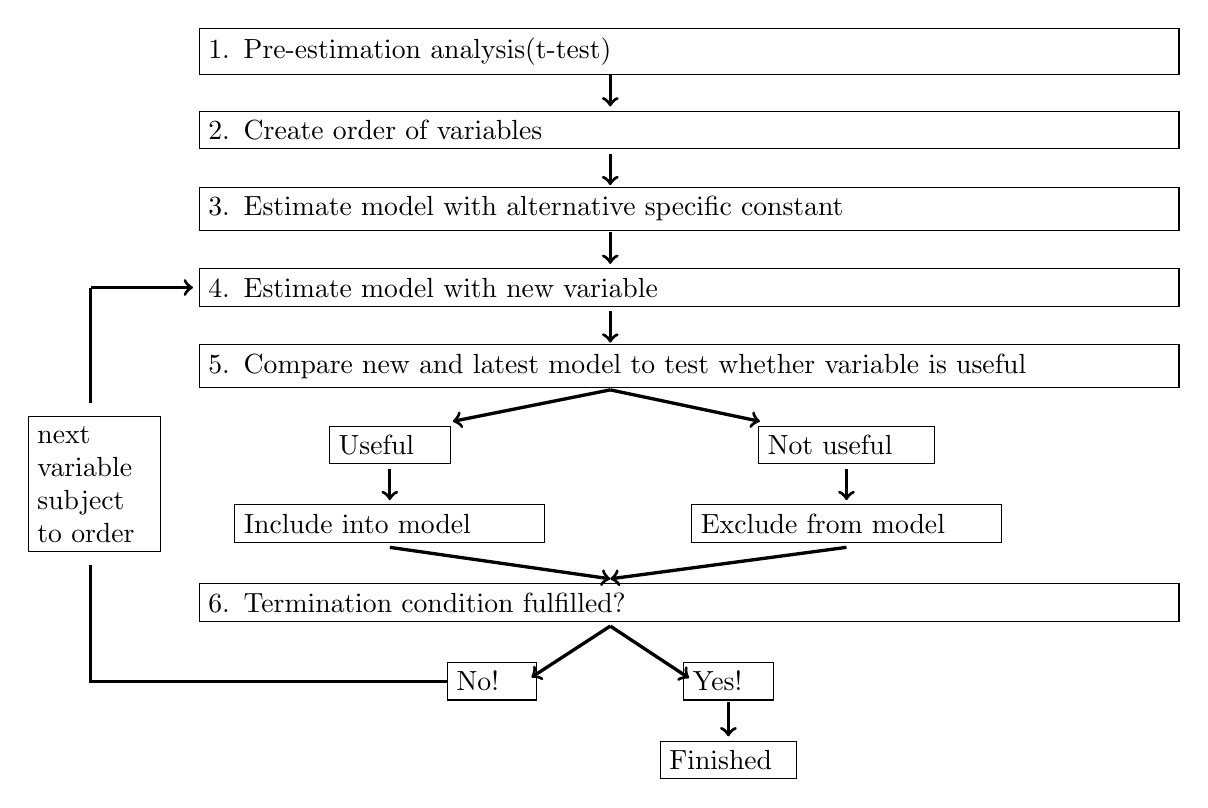
\begin{tikzpicture}
%\draw (0,1.3) node[below] {$B$} --
%(3,1.3) node[below] {$C$};
%\fbox{1.Bestimmung einer Startl\"{o}sung} \\
%\fbox{2.Aktualisierung der Werte} \\
%\fbox{3.Terminierung des Algorithmus}
\node[draw,text width=12.21cm] at (2.5,2){ 1. Pre-estimation analysis(t-test)};
\node[draw,text width=12.21cm] at (2.5,1){ 2. Create order of variables};
\node[draw,text width=12.21cm] at (2.5,0){ 3. Estimate model with alternative specific constant};
\draw [->,very thick] (1.5,1.70) -- (1.5,1.3);
\draw [->,very thick] (1.5,0.7) -- (1.5,0.3);
\draw [->,very thick] (1.5,-0.3) -- (1.5,-0.7);
\draw [->,very thick] (1.5,-1.3) -- (1.5,-1.7);
\draw [->,very thick] (-1.3,-3.3) -- (-1.3,-3.7);
\draw [->,very thick] (4.5,-3.3) -- (4.5,-3.7);
\draw [->,very thick] (1.5,-2.3) -- (-0.5,-2.7);
\draw [->,very thick] (1.5,-2.3) -- (3.4,-2.7);
\draw [->,very thick] (-1.3,-4.3) -- (1.5,-4.7);
\draw [->,very thick] (4.5,-4.3) -- (1.5,-4.7);
\node[draw,text width=12.21cm] at (2.5,-1){4. Estimate model with new variable};
\node[draw,text width=12.21cm] at (2.5,-2){5. Compare new and latest model to test whether variable is useful};
\node[draw,text width=1.3cm] at (-1.3,-3){Useful};
\node[draw,text width=2.0cm] at (4.5,-3){Not useful};
\node[draw,text width=3.7cm] at (-1.3,-4){Include into model};
\node[draw,text width=3.7cm] at (4.5,-4){Exclude from model};
\node[draw,text width=12.21cm] at (2.5,-5){6. Termination condition fulfilled?};
%\draw [-,very thick] (1.5,-1.32) -- (1.5,-1.61);
\node[draw,text width=0.9cm] at (0,-6){No!};
\node[draw,text width=0.9cm] at (3,-6){ Yes!};
\node[draw,text width=1.5cm] at (3,-7){Finished};
\draw [-,very thick] (-0.572,-6) -- (-5.1,-6)-- (-5.1,-4.52);
\draw [-,very thick]  (-5.1,-2.47)-- (-5.1,-1);
\draw [->,very thick] (-5.1,-1) -- (-3.8,-1);
\draw [->,very thick] (1.5,-5.3) -- (0.5,-5.95);
\draw [->,very thick] (1.5,-5.3) -- (2.5,-5.96);
\draw [->,very thick] (3,-6.27) -- (3,-6.70);
\node[draw,text width=1.45cm] at (-5.05,-3.5){next variable subject to order};

\end{tikzpicture}
%\label{fig:dtmc2}
\end{center}
\end{figure}

\vspace{-0.5cm}

\subsection{Estimation Results}

In the following, we use the described method to estimate the model. We
start explaining the method shortly at one iteration. After this, we show the main results considering the estimated probabilities, different predictions methods and a possible extension of the model. \\
%
We start by making the pre-estimation analysis. We detect that the variables "foot", "moveGK" and "GKS" have the highest likelihood of being important for the model. After estimating the model with the alternative specific constants, we start adding step by step the single variables. The first variable we want to include is "foot". By doing the likelihood ratio test to determine whether we should exclude "foot", we get a likelihood-ratio test value of 57.16. As mentioned, the number of restrictions is in this case equal to five. We are to rounded 100 \% confident to reject the hypothesis and include "foot" into our model. This, we can derive from the chi-quadrat values for the different confidence-levels, which we show in the following table.

 \begin{table}[ht]
\caption{Chi-quadrat table}
\centering
\small
\begin{tabular}{ p{3.65cm} |  c |  c |  c }
   Level of confidence number of restrictions & 90\%  & 95\% & 99\%  \\
   \hline

1    &   2.71   & 3.84     & 6.63   \\

2    &  4.61  & 5.99       & 11.34  \\

5    &   9.24   & 11.07    & 15.09  \\

 \end{tabular}
 \end{table}
 
We continue this procedure for all variables on the first list. If the test-value for a variable is at least higher than the 90 \% confidence level, we are including it into the model. The test-values of the variables which we identified as more likely to be important, we show in the following table.


 \begin{table}[ht]
\caption{Likelihood ratio test-values of character-based variables}
\centering
\small
\begin{tabular}{  c |  c | c  | c |  c |  c  }
   variable  & test-value & include in model?  & variable  & test-value & include in model? \\
   \hline

moveGK     & 14.08    &  \checkmark &  tup   & 8.44   &  $\times$   \\ 

GKS       & 14.46   & \checkmark  &  obot      & 8.5    &  $\times$   \\ 

IngSo      & 34.3     & \checkmark  &  Mins3      &6.52    &  $\times$   \\ 

comLea      & 11.06    &  \checkmark &  Mint3   & 5.18    &  $\times$   \\ 

comNTC       & 2.24    & $\times$  &  $la_{3}$     & 11.32    &  \checkmark   \\ 

ClubNT      & 4.16     & $\times$  &  $la_{6}$      & 12.62   &  \checkmark   \\ 

HeiGK      & 10.78    &  \checkmark &  st  & 4.86    & $\times$   \\ 

Imp       & 2.3    & $\times$  &  rnoLS   & 5.38    &  $\times$  \\ 

Dec      & 10.24     & \checkmark  &  Stlsbg      & 4.3    & $\times$   \\ 

lpbg      & 18.78    &  \checkmark &  SlGKd     & 1.06    &  $\times$   \\ 

lGKd       & 4.72    & $\times$  &  Solsbg    & 9.54    &  \checkmark   \\ 


 \end{tabular}
 \end{table}
 
 The variables with a "\checkmark ", we will include into the model. Thus, we include additionally to whether the penalty-taker is left-footed or right-footed ("foot"), whether the match where the penalty is taken, is a "league" match or not ("comLea") and whether the penalty is shot in a penalty shootout or in-match ("IngSo"). Furthermore, regarding a penalty shootout, the fact whether the opponent's last penalty was a goal or not influences the penalty-taker ("Solsbg"). Considering the goalkeeper, his movements during the run-up of the penalty-taker, for instance stepping respectively leaning to a specific side or jumping on spot, are included ("moveGK") as well as his standing position during the run-up ("GKS") and his height (HeiGK). A further big influence is given by the previously shot penalty of the penalty-taker. Especially when the last penalty was shot either to TR or DR ("$la_{3}$", "$la_{6}$") is giving a clue for the next shot direction as well as the fact whether the last penalty was a goal or not ("lpbg"). Last but not least, the fact whether the penalty is a "Decider", we include into our model ("Dec"). \\
%
As a next step, we test which alternative-based variables we will include into the model. We start testing the variable "$SRGK_i$". In the first estimation, by using the same factor for all alternatives, we got a positive value for the factor. Since we assume that the save-rate should get a negative value, since in our opinion it reduces the utility for an alternative, we estimate a factor for each single alternative. For the variable "$MPGK_i$" the same counts theoretically, too. Finally, we include the variables "$SRGK_{TL}$" and "$SRGK_{TR}$", since these have a negative factor and fulfill the likelihood-ratio test condition. Furthermore, we include the \mbox{variable "$perc_i$"}. The other alternative-based variables are excluded from the model. This we conclude by considering the test-values of these variables, which we show in the following table. These test-values, we compare with the corresponding values from \mbox{table 3}. For the variable "$MPGK_i$", we have by testing an individual factor for each alternative five instead of six restrictions, since the alternative DC has no missing probability and so "$MPGK_{DC}$" has no influence on the model. 

\vspace{+0.2cm}
 
  \begin{table}[ht]
\caption{Likelihood ratio test-values of alternative-based variables}
\centering
\small
\begin{tabular}{  c |  c | c |  c  }
   variable & number of added restrictions  & test-value & include in model?   \\
   \hline

"$perc_i$"  & 1 & 6.66   &  \checkmark    \\  

"$SRGK_i$"  & 2  & 7.16    & \checkmark    \\ 

"$MPGK_i$"   & 1 & 0.02  &  $\times$    \\ 

"$MPGK_i$"  & 5 & 5.8    & $\times$    \\ 


 \end{tabular}
 \end{table}
 
 We continue by processing the remaining variables. From these, we include the variable "rnoGroup", which contains the information whether the penalty has shot in a group stage match or not. Furthermore, we include the variable "def", giving the information whether the penalty-taker is a defender or not. Last but not least, the variable "nmovGK" is in our model, which is a further variable considering the movement of the goalkeeper. This variable differs between the goalkeeper is moving or not, but it does not specify the movements, since this is already covered by the variable "moveGK". All other variables like the jersey color, the minute of play, the importance of the game etcetera, we detect as ineffective for predicting. In the following table, we show the final estimations for the different factors of the included variables.
 \\
 \\
 \\
 
  \begin{table}[ht]
\caption{Factors of single utility functions}
\centering
\begin{tabular}{  c |  c | c  | c |  c |  c | c }
   Alt.  & TL & TC  & TR  & DL & DC & DR \\
   \hline

$ASC_i$     & 2.875    &  0.297 &  5.355   & 0.196    &  0 & 2.682  \\ 

$\beta_{foot_i}$  & 0.431    & 0.8033 &  -0.592   & 0.376   &  0 & -0.216  \\ 

$\beta_{moveGK_i}$  & -0.062   & -0.131 & 0.027 & 0.4  &  0 & -0.325   \\ 

$\beta_{GKS_i}$ & 0.241     & 0.019  & -0.589 & -0.162    &  0 & -0.138   \\ 

$\beta_{IngSo_i}$  & -0.214   &  -0.306 &  0.851  & 0.4521  &  0 & 0.231   \\ 

$\beta_{comL_i}$  & -0.696  & -0.484  &  -0.124  & -0.15  &  0 & -0.07   \\ 

$\beta_{HGK_i}$  & 0.048     & 0.019  &  0.016  & -0.015 &  0 & 0.028   \\ 

$\beta_{dec_i}$ & 0.358    &  -1.37 &  0.487  & 0.066    & 0  & 0.193  \\ 

$\beta_{lp_i}$ & 0.076     & -0.577  &  -0.16      & -0.173    & 0 & 0.17   \\ 

$\beta_{latr_i}$  & 0.45   &  0.95  &  1.026   & 0.679    & 0 & 0.538  \\ 

$\beta_{ladr_i}$  & -0.191    &  0.049 &  -0.421   & 0.094   &  0 & -0.226   \\ 

$\beta_{sr_i}$   & -57.185    & 0  &  -134.346   & 0    &  0 & 0   \\ 

$\beta_{perc}$    & 0.333    & 0.333  &  0.333   & 0.333    &  0.333 & 0.333   \\


$\beta_{rnog_i}$   & -0.612    & -0.969  &  0.288  & -0.3    &  0 & -0.232 \\

$\beta_{solsbg_i}$  & 0.104  & -0.6  &  -0.371   & -0.437    &  0 & -0.265  \\

$\beta_{nmovGK_i}$  & 0.01    & -0.475  &  0.222  & 0.61  & 0 & -0.744 \\

$\beta_{def_i}$  & 0.437    & 1.376  &  0.645  & 0.678  & 0 & 0.52 \\

 \end{tabular}
 \end{table}
 
 \vspace{-0.2cm}
 
 Since "DC" is the reference alternative, it has for almost all factors a value \mbox{of 0.} If a factor of a character-based variable has for an alternative a negative sign, this means the variable has a negative utility for this alternative, compared to the reference alternative DC. For example, considering the variable foot, which is for a right-footed player equal to "1" and for a left-footed player equal to "0", the right sided alternatives DR and TR have a negative factor, since right-footed players prefer shooting to the left side. Consequently, the left sided alternatives DL and TL have a positive factor for this variable. Overall, we can use the factors to derive the utility of the respective variables to the single alternatives. \\
For the alternative-based variables, we do not consider a reference alternative. Consequently, for these variables, a negative factor means negative utility and a positive factor means positive utility. The following equations show, exemplarily for the alternative TL, how we construct the utility functions. 
 
 \vspace{-1.2cm}
 
 \begin{center}
 \begin{small}
\begin{align*}
V(TL) &= ASC_{TL} + \beta_{foot_{TL}} \cdot foot + \beta_{moveGK_{TL}} \cdot moveGK  + \beta_{GKS_{TL}} \cdot GKS \\ &+ \beta_{IngSo_{TL}} \cdot IngSo  + \beta_{comL_{TL}} \cdot comLea  + \beta_{HGK_{TL}} \cdot HeiGK + \beta_{dec_{TL}} \cdot Dec \\ &+ \beta_{lp_{TL}} \cdot lpbg  + \beta_{latr_{TL}} \cdot la_{3}  + \beta_{ladr_{TL}} \cdot la_{6} + \beta_{sr_{TL}} \cdot SRGK_{TL} + \beta_{perc} \cdot perc_{TL} \\ &+ \beta_{rnog_{TL}} \cdot rnoGroup  + \beta_{solsbg_{TL}} \cdot Solsbg + \beta_{nmovGK_{TL}} \cdot nmovGK + \beta_{def_{TL}} \cdot def  \\
\end{align*}
\end{small}
\end{center}

 \begin{center}
 \begin{small}
\begin{align*}
V(TL) &= 2.875 + 0.431 \cdot foot - 0.062 \cdot moveGK  + 0.241 \cdot GKS \\ &- 0.214 \cdot IngSo   - 0.696  \cdot comLea  + 0.048 \cdot HeiGK + 0.358 \cdot Dec \\ &+ 0.076 \cdot lpbg  + 0.45 \cdot la_{3}  - 0.191 \cdot la_{6} - 57.185  \cdot SRGK_{TL} + 0.333 \cdot perc_{TL} \\ &- 0.612 \cdot rnoGroup  + 0.104 \cdot Solsbg + 0.01 \cdot nmovGK + 0.437 \cdot def  \\
\end{align*}
\end{small}
\end{center}

\vspace{-1cm}

The other utility functions are construct on the same way. We can use these utility functions to calculate the probabilities for each single alternative given the penalty (conditions). As mentioned, we do this by using the R package apollo. Afterwards, we use the probabilities to predict the shot direction, using two different methods. We predict each single penalty in our database. The prediction results, also considering some single players, we show in the following. \\
%
%


\begin{figure}[ht]
\begin{center}
\caption{Comparison of estimated probabilities}
\begin{minipage}[t]{0.47\linewidth}
  \centering
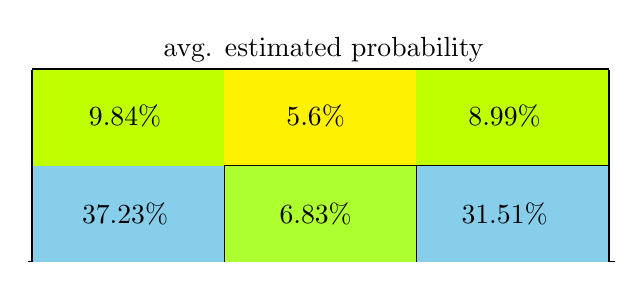
\begin{tikzpicture}
%\draw (0,1.3) node[below] {$B$} --
%(3,1.3) node[below] {$C$};
%\fbox{1.Bestimmung einer Startl\"{o}sung} \\
%\fbox{2.Aktualisierung der Werte} \\
%\fbox{3.Terminierung des Algorithmus}

\draw [-,very thick] (0,2.44) -- (7.32,2.44);
\draw [-,very thick] (0,0) -- (0,2.44);
\draw [-,very thick] (7.32,2.44) -- (7.32,0);
%\draw [-,thick] (-3.66,1.62) -- (3.66,1.62);
\draw [-,thick] (0,1.22) -- (7.32,1.22);
\draw [-,thin] (-0.05,0) -- (7.4,0);


  \path[fill=SkyBlue,draw=black]
        (0,0)
        -- (0,1.22)
        -- (2.44,1.22)
        -- (2.44,0);   
        
       \path[fill=SkyBlue,draw=black]
        (4.88,0)
        -- (4.88,1.22)
        -- (7.32,1.22)
        -- (7.32,0); 
        
        
            \path[fill=GreenYellow,draw=black]
        (2.44,0)
        -- (2.44,1.22)
        -- (4.88,1.22)
        -- (4.88,0); 
        
            \path[fill=lime,draw=black]
        (0,1.22)
        -- (0,2.44)
        -- (2.44,2.44)
        -- (2.44,1.22); 
        
            \path[fill=yellow,draw=black]
        (2.44,1.22)
        -- (4.88,1.22)
        -- (4.88,2.44)
        -- ( 2.44,2.44); 
        
      \path[fill=lime,draw=black]
        (4.88,1.22)
        -- (7.32,1.22)
        -- (7.32,2.44)
        -- (4.88,2.44); 
        
          \draw node[black] at (1.18,1.85) {9.84\%};
  \draw node[black] at (3.6,1.85) {5.6\%};
  \draw node[black] at (6,1.85) {8.99\%};
  \draw node[black] at (1.18,0.61) {37.23\%};
  \draw node[black] at (3.6,0.61) {6.83\%};
  \draw node[black] at (6,0.61) {31.51\%};
  \draw node[black] at (3.7,2.7) {avg. estimated probability}; 

\end{tikzpicture}
\end{minipage}
\hfill
\begin{minipage}[t]{0.47 \linewidth}
\centering
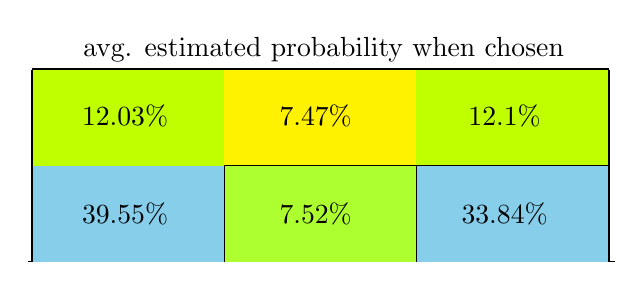
\begin{tikzpicture}
%\draw (0,1.3) node[below] {$B$} --
%(3,1.3) node[below] {$C$};
%\fbox{1.Bestimmung einer Startl\"{o}sung} \\
%\fbox{2.Aktualisierung der Werte} \\
%\fbox{3.Terminierung des Algorithmus}

\draw [-,very thick] (0,2.44) -- (7.32,2.44);
\draw [-,very thick] (0,0) -- (0,2.44);
\draw [-,very thick] (7.32,2.44) -- (7.32,0);
%\draw [-,thick] (-3.66,1.62) -- (3.66,1.62);
\draw [-,thick] (0,1.22) -- (7.32,1.22);
\draw [-,thin] (-0.05,0) -- (7.4,0);


  \path[fill=SkyBlue,draw=black]
        (0,0)
        -- (0,1.22)
        -- (2.44,1.22)
        -- (2.44,0);   
        
       \path[fill=SkyBlue,draw=black]
        (4.88,0)
        -- (4.88,1.22)
        -- (7.32,1.22)
        -- (7.32,0); 
        
        
            \path[fill=GreenYellow,draw=black]
        (2.44,0)
        -- (2.44,1.22)
        -- (4.88,1.22)
        -- (4.88,0); 
        
            \path[fill=lime,draw=black]
        (0,1.22)
        -- (0,2.44)
        -- (2.44,2.44)
        -- (2.44,1.22); 
        
            \path[fill=yellow,draw=black]
        (2.44,1.22)
        -- (4.88,1.22)
        -- (4.88,2.44)
        -- ( 2.44,2.44); 
        
      \path[fill=lime,draw=black]
        (4.88,1.22)
        -- (7.32,1.22)
        -- (7.32,2.44)
        -- (4.88,2.44); 
        
          \draw node[black] at (1.18,1.85) {12.03\%};
  \draw node[black] at (3.6,1.85) {7.47\%};
  \draw node[black] at (6,1.85) {12.1\%};
  \draw node[black] at (1.18,0.61) {39.55\%};
  \draw node[black] at (3.6,0.61) {7.52\%};
  \draw node[black] at (6,0.61) {33.84\%}; 
  
  \draw node[black] at (3.7,2.7) {avg. estimated probability when chosen}; 

\end{tikzpicture}
\end{minipage}
\end{center}
\end{figure}

We first show in figure 7 on the left side the average probabilities of each single alternative estimated by our model. Comparing this to figure 3, we can observe that the average probabilities are exactly like the probabilities of our database. On the right side, we show the estimated average probabilities of the single alternatives, in the case they are chosen by the penalty-takers. Comparing these to the left side, we can observe that our models estimates these probabilities for all alternatives clearly higher. This is especially valid for the shots to the right or to the left, for which the increase is at least 2.19 \%. Consequently, our model is able to recognize some patterns and variables increasing the utility of the single alternatives.  \\
In the next step, we give an analysis of some single players. The figure 8 shows the estimated average probabilities for each alternative of the players Griezmann, Dybala, Suarez and Ramos.
\\

\begin{figure}[ht]
\begin{center}
\caption{Estimated average probabilities of different penalty-takers}
\begin{tikzpicture}[scale = 0.9]
\begin{axis}[
width=15cm, height =10.4cm,
ybar,enlargelimits=0.15,
symbolic x coords={TL,TC,TR,DL,DC,DR},xtick={TL,TC,TR,DL,DC,DR},
legend style={
  at={(current bounding box.south-|current axis.south)},
  anchor=north,
  legend columns=-1
},
]

\addplot+[fill=blue] coordinates
{(TL,7.14) (TC,3.45) (TR,16.89)(DL,27.37) (DC,5.9) (DR,39.23)};
\addplot +[fill=pink] coordinates 
{(TL,6.722) (TC,3.179) (TR,11.44)(DL,29.69) (DC,6.5) (DR,42.46)};
\addplot +[fill=yellow] coordinates
{(TL,10.07) (TC,6) (TR,6.28)(DL,39.95) (DC,6.8) (DR,30.89)};
\addplot +[fill=TealBlue] coordinates
{(TL,9.07) (TC,13.03) (TR,6.74)(DL,41.78) (DC,3.42) (DR,25.96)};

\node[rotate=90, blue] at(-31.5,77.14){7.14 $\%$};
\node[rotate=90, red] at(-10.5,72.14){6.72 $\%$};
\node[rotate=90, black] at(9.5,114.14){10.07 $\%$};
\node[rotate=90, teal] at(29.5,98.14){9.07 $\%$};

\node[rotate=90, blue] at(67.5,40.14){3.45 $\%$};
\node[rotate=90, red] at(90,38.74){3.18 $\%$};
\node[rotate=90, black] at(110,67.14){6.00 $\%$};
\node[rotate=90, teal] at(130,143.14){13.03 $\%$};

\node[rotate=90, blue]  at(168,182){16.89 $\%$};
\node[rotate=90, red]   at(190,127){11.44 $\%$};
\node[rotate=90, black] at(210,69){6.28 $\%$};
\node[rotate=90, teal]  at(230,73){6.74 $\%$};

\node[rotate=90, blue]  at(269,287){27.37 $\%$};
\node[rotate=90, red]   at(290,312){29.69 $\%$};
\node[rotate=90, black] at(310,411){39.95 $\%$};
\node[rotate=90, teal]  at(330,417){41.78};

\node[rotate=90, blue]  at(368,62){5.9 $\%$};
\node[rotate=90, red]   at(390,66){6.5 $\%$};
\node[rotate=90, black] at(410,70){6.8 $\%$};
\node[rotate=90, teal]  at(430,41){3.42 $\%$};

\node[rotate=90, blue]  at(468,406){39.23 $\%$};
\node[rotate=90, red]   at(490,422){42.46};
\node[rotate=90, black] at(510,320){30.89 $\%$};
\node[rotate=90, teal]  at(530,272){25.96 $\%$};

\legend{Griezmann(32;L;ST),Dybala(28;L;ST),Suarez(58;R;ST),Ramos(40;R;DF)}


\end{axis}
\end{tikzpicture} 
\end{center}
\end{figure}

\vspace{+0.1cm}

In brackets, we show the number of penalties in the database, the strong foot and the position of the single players. We can clearly observe that our model differs extremely between left-footed and right-footed players. For Griezmann and Dybala our model estimates a clearly higher probability to shoot to the right of the goal than for Suarez and Ramos and vice versa, for Suarez and Ramos our model estimates a higher probability to shoot to the left. Furthermore, we can observe that the players Griezmann and Dybala, which have the same position and the same strong foot, have also relative similar estimated probabilities. Nevertheless, the probabilities are especially for the alternatives DL, DR and TR not equal, so the model differentiates between these two players.\\
Considering the example, the player Ramos has the biggest estimated average probability for the alternative TC, which is more than twice as high as for the other players. The reason for that is, that this player more often shoots to that direction (30 \% in db). Our model is able to recognize this, cause of using the \mbox{variable "$perc_i$"}. The same accounts for the player Griezmann, who more often shoots to the right upper corner (31.25\% in db), and so he gets a relative high estimated average probability for this alternative. Nevertheless, our model just rarely predicts these alternatives as the alternative with the highest probability, which we show in the following. 

\subsection{Prediction Results} 

We first start by using the prediction method according to our mathematical model. The alternative with the highest utility, meaning the alternative with the highest probability, is our prediction. Overall, using this method we are able to predict \mbox{42.24 \%} of the penalties correctly and vice versa \mbox{57.76 \%} incorrect. This is clearly better than predicting for each penalty it will be shot to "DL", the alternative with the highest probability, which would give us a prediction rate of 37.23 \% correct predictions. Additionally, we show in table 7 how often in the database the single alternatives are chosen, how often the alternatives have according to our model the highest probability and how often in that case the ball was shot to that direction. 


  \begin{table}[ht]
\caption{Numbers of choice considering the alternatives}
\centering
\small
\begin{tabular}{  c |  c | c | p{5cm}  }
   alt. & times chosen (db) & times highest probability & times chosen by penalty-taker when highest probability   \\
   \hline

TL  & 232 &  12  &  5    \\  

TC  & 132  & 1    & 0    \\ 

TR   & 212 & 20  &  7    \\ 

DL  & 878 & 1606    & 678    \\ 

DC  & 161 & 0   &  -    \\ 

DR  & 743 & 719   &  306    \\ 

 \end{tabular}
 \end{table}
 
 \vspace{-0.2cm}
 
As an example, when our model predicts "DR", it is in 42.56\% of the cases correctly. Our models rarely predicts a shot to the top of the goal (33 times). Furthermore, shooting to the center of the goal has only one time the highest probability using our model. This is clearly dominated by the alternatives DL and DR, which is obvious, since these alternatives are the most chosen. However, if a penalty-taker knows that a goalkeeper is behaving according to our prediction method, he just would shoot to the center of the goal and has a great chance to score a goal. Since this scenario would make our model ineffective, we create a further prediction method. \\
According to this method, we calculate for each alternative the difference of the estimated probability ($Pr_i$) and the estimated average probability ($\overline{Pr_i}$). We then choose the alternative with the maximum difference. This alternative has the highest increase in probability respectively utility. For this method, the same assumptions and equations are valid as we presented in the mathematical model (section 4.1). We only change the assumption, which alternative we choose (equation 1). 

\vspace{-1.35cm}

 \begin{center}
 \begin{align}
 C = \{ i | (Pr_i - \overline{Pr_i}) = max(Pr_i - \overline{Pr_i}) \}
 \end{align}
 \end{center}
 
 \vspace{-0.35cm}
 
 An example for the method, regarding a random penalty, we show in the next table.

  \begin{table}[ht]
\caption{Example second prediction method}
\centering
\small
\begin{tabular}{  c |  c | c |  c | c | c | c  }
   alternative & TL  & TC & TR & DL & DC & DR   \\
   \hline

estimated prob.  & 0.128 &  0.043  &  0.203  & 0.24 & 0.074 & \textcolor{teal}{0.3116}    \\  

avg. prob.  & 0.098  & 0.056    & 0.09 & 0.372 & 0.068 & 0.3151    \\ 

\hline

increase in prob.   & 0.03  & -0.013  &  \textcolor{blue}{0.113} & -0.132 & 0.006 & -0.0035    \\ 

 \end{tabular}
 \end{table}
 
 \vspace{-0.2cm}
 
 In the example, TR has the highest increase in probability and DR has the highest overall probability. Consequently, we predict TR instead of DR. The advantage of this method is that we predict all alternatives frequently. We choose 62 times DC and 177 times TC, which is clearly more than one time. Our prediction is 805 times DL, which is almost the half compared to the first method. Furthermore, we predict 663 times DR, 377 times TL and 274  times TR. We can observe that this distribution is clearly more balanced, and more similar to the quantity the alternatives are chosen in the database. The disadvantage of the method is a low prediction rate of \mbox{33.59 \%,} which is almost 9 \% less compared to the first method. \\
%
Consequently, a combination of both methods could be interesting. On the one hand, this would enable a relative high prediction rate. On the other hand, each alternative would be predicted sometimes. A possible method for this is to predict using the second method if and only if the probability increase is greater than a specific boundary. As example, we use an alternative-specific boundary (B), calculated for each alternative by the maximum estimated probability (max($Pr_i$)) reduced by the average estimated probability ($\overline{Pr_i}$) and this result divided \mbox{by 2.5}. We got this boundary via testing.
 
 \vspace{-2cm}
 
 \begin{center}
 \begin{align}
 B = \frac{max(Pr_i) - \overline{Pr_i}}{2.5}
 \end{align}
 \end{center}
 
 \vspace{-0.1cm}

Using the combined methods and this boundary, we are predicting in 40.63 \% of the cases correctly. This is a strong increase compared to the second method. We predict 57 times DC, 16 times TC, 97 times TL and 29 times TR. Compared to the numbers of table 12, we clearly more often predict these rather unusual alternatives. Overall, we need to weigh up, which requirements we want to have for our predictions and choose according to these requirements a suited method. \\
%
Last but not least, we shortly investigate the prediction rate of penalty-taker that have only one shot in our database and those that have at least five penalties, using the first prediction method only. We present this in the following table, whereby we always show the average prediction rate of all penalty-takers with the according number of penalties in our database.

  \begin{table}[ht]
\caption{Prediction rate of penalty-takers with different number of penalties}
\centering
\small
\begin{tabular}{  c |  c | c | c | c | c }
   number of penalties & 1 &  5-9 & 10-29  & 30-49  & 50 or more    \\
   \hline

perc. correct  & 35.49\% &  37,76\%  &  42.36\%  & 46.63\% & 43.95\%    \\  

 \end{tabular}
 \end{table}
 
We observe that the prediction rate of 35.49 \% for penalty-takers with only one penalty is relative small. The higher the number of considered penalties for a single player, the higher is the prediction rate. The only exception is for penalty-takers with over 50 penalties, for which we still have a relative high prediction rate. Since we can observe more penalties and several variables in our model consider the previously shot penalties of a penalty-taker, the increase in prediction rate by an increasing number of penalties considered, is reasonable. Consequently, if we want to predict the behavior of a penalty-taker, we should collect as much penalty-data of that player as we can. Nevertheless, even for the penalty-takers for which we collect a lot of data, we predict on average under 50\% correctly, thus less than a half. Concluding, we can state that predicting the shot direction is a difficult task.

As a potential extension of our model, we consider building a nested multinomial logit model. A detailed description of this model is given by \mbox{Koppelman \& Bhat (p.157f)}. The main advantage of this model is to avoid the independence of irrelevant alternative's assumption we make by the multinomial logit model. Therefor, we build nests/subgroups of alternatives, which are relative similar to each other. We regard building the nests by separating the goal vertically into left (TL and DL), center (TC and DC) and right (TR and DR). We assume that the most influencing variables are the same as for the normal MNL. Furthermore, we assume that the utility functions are almost the same. The only difference is that the alternatives belonging to the same nest, we decide to have the same \mbox{($\beta$-) factor} of the variable "foot". \\
 Overall, this extension gives no observable improvement to the normal model. The prediction rate using the highest utility method is 41.86 \%, which is very similar to our normal MNL. The "problem" of predicting the rather unusual alternatives infrequently, we have by using this nested model, too. Important to state is that the nested variant is computational expensive, and we reach the maximum number of iterations the software is in our case able to execute. Consequently, we are not able to fully investigate this kind of model and stop further investigations.


\section{Conclusion}

Summarizing, we present a discrete choice model which can help to predict the behavior of a penalty-taker in soccer. Using our model, we can answer the questions arose in the beginning of this thesis. In this thesis, we first showed how we derive suitable, high-quality data of overall 2358 different penalties. This process includes to find possible factors influencing the decision, where to shoot the ball. Collecting and preparing the data are further steps in this process. \\
Afterwards, we described the way we want to estimate a suited model, and we then presented our results. All in all, the footedness of the penalty-taker and the previous behavior by penalties (especially considering the last penalty) are the main influencing variables of predicting the behavior. Regarding the goalkeeper, the position in the goal and the movement, both during the run-up to the penalty, have a big impact on the penalty-taker. The height of the goalkeeper influences the penalty-taker, too. Moreover, we show that the kind of competition, e.g. a league match, can help to predict. Last but not least, the behavior of the penalty-taker can differ when a penalty is shot in a penalty shootout.  \\
Using our model, we derive the probabilities where a penalty-taker most likely shoots a penalty. Moreover, we compare the estimated probabilities of different players to display how our models differs between different and relative equal types of penalty-taker. We further show how to predict the shot direction using our model. There we present two methods, where one has a higher accuracy, but only one time predicts for the goalkeeper to stay in the center. The other one has a clearly lower accuracy, but we predict each shot direction frequently. Furthermore, we show that the more penalty data we have for a specific penalty-taker, mostly the better we are able to predict him. \\
All in all, we can state that predicting the behavior of a penalty-taker is very difficult. Regarding that some penalty-takers observe the movement of the goalkeeper shows that the penalty-takers are able to make their decision where to shoot the ball in just a few seconds. Consequently, a penalty-taker is able to change his desired shot direction during his run-up, which is a possible reason why predicting gets hard. \\
For future research, we could search for different methods to predict the shot direction using our model respectively our calculated probabilities. Moreover, we could investigate whether we find further variables influencing the behavior of the penalty-taker significantly. Generally, the main limitations of our data is that it is video analyzed manually by a human, which never can be as accurate as when this is done by a computer. Using technology could give further improvements and gives the possibility to investigate further factors like the velocity of the ball or the posture and the line of gaze of the penalty-taker, too. \\
Moreover, the investigations considering the nested multinomial logit model could be continued. The number of different nests is very high, even though not all potential pairs of alternatives seem to be logically reasonable. Nevertheless, the nested models have advantages, for which further investigations can be interesting. 


%%%%%%%%%%%%%%%%%%%%%%%%%%% Literaturverzeichnis %%%%%%%%%%%%%%%%%%%%%%%%%%%%%%%%
\newpage
\newpage
\clearpage
\pagenumbering{Roman}
\setcounter{page}{5}

\begin{thebibliography}{99}
\markboth{References}{References}
\addcontentsline{toc}{section}{\vspace{1pt}References}

\harvarditem{Almeida}{2016}{Almeida} Almeida, C.H.; Volossovitch, A.; Duarte, R. (2016). Penalty kick outcomes in UEFA club competitions (2010-2015): The roles of situational, individual and performance factors. International Journal of Performance Analysis in Sport 16, 508-522.
%\harvarditem{Andersen}{2011}{Andersen} Andersen, T.; D\"orge, H.C. (2011) The influence of speed of approach and accuracy constraint on the maximal speed of the ball in soccer kicking. Scandinavian Journal of Medicine and Science in Sports 21(1):79-84.
%\harvarditem{Azar}{2011}{Azar} Azar O.H.; Bar-Eli, M. (2011) Do Soccer Players Play the Mixed-Strategy Nash Equilibrium. Applied Economics, 43 (25-27), 3591-3601
%\harvarditem{Bar-Eli}{2009}{Bar-Eli} Bar-Eli, M.;  Azar O.H. (2009) Penalty kicks in soccer: An empirical analysis of shooting strategies and goalkeepers' preferences. Soccer and Society, 10(2), 183-191
\harvarditem{Baumann}{2011}{Baumann} Baumann, F.; Friehe, T.; Wedow, M. (2011). General Ability and Specialization: Evidence From Penalty Kicks in Soccer. Journal of Sports Economics 12(1), 81-105
\harvarditem{Buzzacchi}{2014}{Buzzacchi} Buzzacchi L.; Pedrini S. (2014). Does player specialization predict player actions? Evidence from penalty kicks at FIFA World Cup and UEFA Euro Cup. APPLIED ECONOMICS, 46(10), 1067-1080.
\harvarditem{Chiappori}{2002}{Chiappori} Chiappori, P.A.; Levitt, S.; Groseclose, T. (2002) Testing Mixed-Strategy Equilibria When Players Are Heterogeneous: The Case of Penalty Kicks in Soccer. American Economic Review 92, 1138-1151
\harvarditem{Dalton}{2015}{Dalton} Dalton, K.; Guillon, M.; Naroo, S.A. (2015). An Analysis of Penalty Kicks in Elite Football Post 1997. International Journal of Sports Science \& Coaching 10(5), 815-827
\harvarditem{Hess}{2021}{Hess} Hess, S.; Palma, D. (2021). Apollo: a flexible, powerful and customisable freeware package for choice model estimation and application. version 0.2.4; Choice Modelling Centre, University of Leeds. Available online: http://www.apollochoicemodelling.com/files/Apollo.pdf; last manual edit: 29.03.21
\harvarditem{Hess}{2021}{Hess} Hess, S.; Palma, D. (2021). example codes, available online: http://www.apollochoicemodelling.com/index.html
\harvarditem{Horn}{2020}{Horn} Horn, M.; de Waal, S.; Kraak, W. (2020). In-match penalty kick analysis of the 2009/10 to 2018/19 English Premier League competition. International Journal of Performance Analysis in Sport, 21, 139-155
\harvarditem{Hughes}{2002}{Hughes} Hughes, M.; Wells,J. (2002). Analysis of penalties taken in shoot-outs. International Journal of Performance Analysis in Sport 2(1)55-72.
\harvarditem{Jordet}{2007}{Jordet} Jordet, G.; Hartmann, E.; Visscher, G.; Lemmink, K.A.P.M (2007). Kicks From the Penalty Mark in Soccer: The Roles of Stress, Skill, and Fatigue For Kick Outcomes. Journal of Sports Sciences 25(2), 121-129.
\harvarditem{Koppelman}{2006}{Koppelman} Koppelman, F.S.; Bhat, C. (2006). A Self Instructing Course in Mode Choice Modeling: Multinomial and Nested Logit Models. U.S. Department of Transportation., Available online: \small{https://www.caee.utexas.edu/prof/bhat/COURSES/LM\_Draft\_060131Final-060630.pdf}
%\harvarditem{Kerwin}{2006}{Kerwin} Kerwin, D.G.; Bray, K. (2006). Measuring and Modelling the Goalkeeper's Diving Envelope in a Penalty Kick. Found in: The Engineering of Sport 6 (2006), Volume 1 Development for Sports, 321-326.
\harvarditem{Krumer}{2016}{Krumer} Krumer, A. (2020). Pressure versus ability: Evidence from penalty shoot-outs between teams from different divisions. Journal of Behavioral and Experimental Economics 89, 101578
\harvarditem{Lidor}{2012}{Lidor} Lidor, R.; Ziv, G.; Gershon, T. (2012) Psychological Preparation of Goalkeepers for the 11-m Penalty Kick in Soccer - A Review. Sport Psychologist, 26(3), 375-389.
\harvarditem{Muller}{2018}{Muller} M\"uller, F.; Best, J.F.; Canal-Bruland, R. (2018). Goalkeepers Reputations Bias Shot Placement in Soccer Penalties. Journal of Sport and Exercise Psychology, 40, 128-134.
\harvarditem{Navarro}{2013}{Navarro} Navarro, M.; van der Kamp, J.; Ranvaud, R.; Savelsberg, G.J.P. (2013) The mere presence of a goalkeeper affects the accuracy of penalty kicks. Journal of Sports Sciences, 31(9), 921-929.
\harvarditem{Noel}{2015}{Noel} Noel,B.; Furley, P.; van der Kamp, J.; Dicks, M.; Memmert, D. (2015) The development of a method for identifying penalty kick strategies
in association football. Journal of Sports Sciences, 33(1), 1-10
\harvarditem{Noel}{2015}{Noel} Noel, B.; Furley, P.; H{\"u}ttermann, S.; Nopp, S.; Vogelbein, M.; Memmert, D. (2014). Einflussfaktoren auf Erfolg und Misserfolg beim Elfmeterschie\ss{}en:
Eine empiriegeleitete retrospektive Analyse der Europa- und Weltmeisterschaften von 1982 bis 2012, Zeitschrift f{\"u}r Sportpsychologie, 21, 51-62 
\harvarditem{Wood}{2010}{Wood} Wood, G.; Wilson, M.R. (2010). A moving goalkeeper distracts penalty takers and impairs shooting accuracy. Journal of Sports Sciences, 28(9), 937-946.


\end{thebibliography}  

\newpage

\large{\textbf{References Data Sources}}

\vspace{+0.5cm}

 \begin{table}[h]
\caption{List of data sources}
\centering
\begin{tabular}{ p{3.15cm} | p{11.15cm}  }
    $area$ & $source$   \\
   \hline

sources regarding player and match facts & www.transfermarkt.de; www.kicker.de; www.sport.de; www.bundesliga.de; www.spox.com; www.fifa.com; www.ran.de; www.sky.de; www.torwart.de; www.eplreview.com; www.iffhs.com; www.weltfussball.de; www.fussballdaten.de  \\

video sources (publisher)\footnotemark[4] & Sportschau.de; Bild.de; Dazn; Sportbild.de; Bundesliga.de; Sky.Sport; DFB.de; official YouTube channels of: (publisher mentioned before; Serie A ; LaLiga Santander; \mbox{Ligue 1}; Premier League; Sky Sport HD; RptimaoTV;  Manchester United; Tottenham Hotspurs; AC Milan; FC Bayern M{\"u}nchen; FC Barcelona; Real Madrid; Liverpool FC; Inter Mailand; SSC Neapel; Paris St.Germain; Lazio Rom; Juventus Turin; Athletico Madrid; AS Rom; FC Porto; Sporting Lissabon; Sport TV; VSPORTS; Sportstudio; Uefa.com; FIFATV; Copa America; CAF TV);  YouTube; Dailymotion; VSPORTS

 \end{tabular}
 
\vspace{+0.5cm}
 
\footnotemark[4] During working and writing on the thesis, some videos used for collecting the 
 \newline 
 \hspace*{-91mm} data got  unavailable online. 
 
 \end{table}

 \pagebreak


\begin{table}[h]
\caption{Variable description \small{I}}
\centering
\begin{tabular}{ c | p{13cm}  }
    $Variable$ & $Description$   \\
   \hline
	
ppos & penalty-taker's position. Coding; 0: Goalkeeper, 1: Defender, 2: Midfielder, 3: Striker. The same player has always the same position, even if in a match where the player shoots a penalty he plays on another position. For wingers we decide in the individual case whether striker or midfielder  \\

def & whether penalty-taker is defender or not. Coding; 0:no, 1:yes \\

mf & whether penalty-taker is midfielder or not. Coding; 0:no, 1:yes \\

st & whether penalty-taker is striker or not. Coding; 0:no, 1:yes \\

foot & strong foot of penalty-taker. Coding; 0: Left, 1: Right  \\

Age & Age of penalty-taker, coding type. Coding; 1: age$<$21, 2: 22, 3: 23, 4: 24, 5: 25, 6: 26, 7: 27, 8: 28, 9: 29, 10: 30, 11: 31, 12: 32,  13: 33, 14: age$>$33  \\

RepGK & Goalkeeper with great Reputation. Coding; 0: no, 1: yes. Chosen Goalkeeper:  Alisson, Barthez, Bravo, Buffon, Carrasso, Casillas, Cech, Consigli, Costil,  Courtois, Diego Alves, Donnarumma, F\"ahrmann,  Handanovic, Hart, Jimenez,  Julio Cesar, Krul, Lloris, Navas, Neuer, Oblak, Rafael, Schmeichel, Simon, Sirigu, Subasic, Szczesny, ter Stegen, Viviano, choice based on article\footnotemark[5] and the choice of the world's best goalkeeper done by the FIFA and IFHHS  \\
 
HeiGK & Height of Goalkeeper [in cm]. Coding; 1: height$<$183, 2: 183, 3: 184, 4: 185,  5: 186, 6: 187, 7: 188, 8: 189, 9: 190, 10: 191, 11: 191, 12: 193, 13: 194, 14: 195, 15: 196, 16: height$>$196  \\

tpos & table position of club of penalty-taker. Coding; 0/NA: no table position available, 1: upper, 2: middle, 3: bottom. upper: approx. upper third of the table ; middle: approx. second third of the table; bottom: approx. down third of the table \\

tup & whether team of penalty-taker is on a upper place of the table or not. Coding; 0/NA: not available, 1: no, 2: yes \\

tmid & whether team of penalty-taker is on a middle place of the table or not. Coding; 0/NA: not available, 1: no, 2: yes \\

tbot & whether team of penalty-taker is on a bottom place of the table or not. Coding; 0/NA: not available, 1: no, 2: yes \\
 
otpos & table position of opponent of penalty-taker. Coding; 0/NA: no table position available, 1: upper, 2: middle, 3: bottom. same structure as for "tpos"  \\

oup & whether opponent of penalty-taker is on a upper place of the table or not. Coding; 0/NA: not available, 1: no, 2: yes \\

omid & whether opponent of penalty-taker is on a middle place of the table or not. Coding; 0/NA: not available, 1: no, 2: yes \\

obot & whether opponent of penalty-taker is on a bottom place of the table or not. Coding; 0/NA: not available, 1: no, 2: yes \\
 
 \end{tabular}
  \vspace{+0.5cm}
  
 \small{\footnotemark[5] https://www.spox.com/de/sport/fussball/international/1912/Diashows/gehaltene-\\ \ \ \ elfmeter-seit-2010/elfmeterkiller-des-jahrzehnts-dieser-keeper-hielten-die-meisten
 \newline \hspace*{-112mm} -elfmeter.html }
 \end{table}

 \pagebreak

\begin{table}[h]
\caption{Variable description \small{II}}
\centering
\begin{tabular}{ c | p{12cm}  }
    $Variable$ & $Description$   \\
   \hline

fav & being favourite or underdog in a match based on league and table position. \newline 1: underdog, 2: same level, 3: slightly favourite, 4: one league higher, 5: two or more leagues higher. As "slightly favourite" we define matches against teams playing in the same league, but the team of the penalty-taker is at least 10 places better in the table than the opponent. This is not valid for matches before the 6th matchday of a season. These matches we assume to have no favourite. A team is an "underdog" if its opponent plays in a higher conference or the opponent is a "slightly favourite". For national teams we derive being a favourite by regarding the official Fifa World Ranking, rank difference 1-30 = no favourite, rank difference 31-60  = slighlty favourite/underdog,  rank difference 60-120 is like one league difference, rank difference 120 or higher is like two leagues difference \\

favU & whether team of penalty-taker is the underdog before kickoff or not. Coding; 0: no, 1: yes \\

favF & whether team of penalty-taker is the favourite (including fav=3v4v5) before kickoff or not. Coding; 0: no, 1: yes \\	

loc & location of match. Coding; 1: Home, 2: Neutral, 3: Away  \\

locH & whether team of penalty-taker is playing at home or not. Coding; 0: no, 1: yes \\

locN & whether team of penalty-taker is playing on neutral location or not. Coding; 0: no, 1: yes \\

locA & whether team of penalty-taker is playing away or not. Coding; 0: no, 1: yes \\

rnoGroup & whether team of penalty-taker is playing in a group stage match or not. Coding; 0: no, 1: yes \\

rko & whether team of penalty-taker is playing in a "Last sixteen", in a quarter-final, in a semi-final or final match or not. Coding; 0: no, 1: yes \\

IngSo & whether penalty is shot in-match or in a penalty shootout. Coding; 0: Ingame, 1: shootout \\

Min & Minute when penalty given. Coding; 0/NA: shootout/not available, 1: Minute $<$ 16, 2: 15 $<$ Minute $<$ 31, 3: 30 $<$ Minute $<$ 46, \newline 4: 45 $<$ Minute $<$ 61, 5: 60 $< $Minute $<$ 76 \& 90 $<$ Minute $<$ 106, 6: 75 $<$ Minute $<$ 90 \& 105 $<$ Minute $<$ 120, \newline  7:  Minute $=$ 90 \& Minute $=$ 120 \\

Minf3 & whether penalty is in the first thirty minutes of match. Coding; 0/NA: not available, 1: no, 2: yes \\

Mins3 & whether penalty is in the second thirty minutes of match. Coding; 0/NA: not available, 1: no, 2: yes \\

Mint3 & whether penalty is in the third thirty minutes of match or in the overtime (not including the 90th and 120th minute). Coding; 0/NA: not available, 1: no, 2: yes \\

Min90 & whether penalty is in the 90th or 120th minute. Coding; 0/NA: not available, 1: no, 2: yes \\

 \end{tabular}
 \end{table}

\pagebreak

\begin{table}[h]
\caption{Variable description \small{III}}
\centering
\begin{tabular}{ c | p{12cm}  }
    $Variable$ & $Description$   \\
   \hline

Imp & Importance of match. Coding; 1: unimportant, 2: normal, 3: important.  is derived for each match individually and is determined slightly subjectively. As rule of thumb: each match played in the league, the first three rounds of each "cup" or each match during a group stage have a "normal" importance. Friendly games and the last matchdays of a season or group stage, where the team is not able to win or lose a place in the table are defined as "unimportant". \linebreak "important":  League matches can be important if it is a special match (e.g. against a rival) or if the match is within the last ten matchdays of a season and the team is playing against a direct opponent in the table. Especially matches of the last three matchdays of a season, when a team is playing against relegation or for a place qualifying to the "Champions League" or "Europa League", can be determined as "important", even though the opponent is no direct competition.  For each competition using a knockout system, we define each match played in the round of the last sixteen, quarter final, semi final and the final as "important". The importance of qualifications matches we assess depending on three factors: team is already qualified $\rightarrow$ unimportant , normal qualification match $\rightarrow$ "normal" importance, qualification match in ko-system or last possible match to qualify $\rightarrow$ important.  \\

Dec & whether penalty is deciding (based on short time remaining). Coding; 0: no, 1: yes. A "Decider" is in an ingame-match a penalty shot in the 90th minute, which would change the actual result crucially to a draw or to a lead, in case of the penalty is scored. Potential additional time is not investigated for this, meaning the "Decider" is not necessarily the last action of a match and further goals can be scored even after a "Decider". Regarding penalty shootouts there are two cases defining a "Decider". The first case is when the penalty-taker scores the penalty his team is winning the match. The second case is when the penalty-taker is not scoring the penalty, his team is losing the match. \\


SpecM & whether match is a special match. Coding; 0: no, 1: yes. Based on the opponent team. As Special Match we define matches against the top teams of each league, international top teams, the top national teams and each match known as "derby"\footnotemark[6], where a team is playing against his rival. Teams with * we assume to be international top teams, the rest are top teams of their league,  List: FC Bayern M{\"u}nchen(*), Borussia Dortmund ,Atletico Madrid, FC Barcelona(*), Real Madrid(*), Benfica Lissabon, Sporting Lissabon, Juventus Turin(*), Manchester City(*), Manchester United(*), Liverpool FC(*), Chelsea London,  Italy, France, Spain, Germany, Portugal, Brazil, Argentina, England, Netherlands\\


 \end{tabular}
 
 \vspace{+0.5cm}
 
 \footnotemark[6] list of rivals/derbys derived from the video game Football Manager 2021; \newline  \hspace*{-3mm} Developer: Sports Interactive, Publisher: Sega, licenses of overall 29 
 \newline \hspace*{-123mm} leagues 
 
 \end{table}

\pagebreak
 
 \begin{table}[h]
\caption{Variable description \small{IV}}
\centering
\begin{tabular}{ c | p{12cm}  }
    $Variable$ & $Description$   \\
   \hline 
   
iLdbb & actual result when penalty is taken (lead, draw, in behind). Coding; 1: behind by 3 or more (goals), 2: behind by 2, 3: behind by 1; 4: draw, 5: in lead by 1, 6: in lead by 2 or more \\

bb2 & whether team of penalty-taker is actually in deficit by two or more goals. Coding; 0: no, 1: yes \\

bb1 & whether team of penalty-taker is actually in deficit by one goal. Coding; 0: no, 1: yes \\

d0 & whether actual result is a draw. Coding; 0: no, 1 :yes \\

il1 & whether team of penalty-taker is actually in lead by one goal. Coding; 0: no, 1: yes \\

il2 & whether team of penalty-taker is actually in lead by two or more goals. Coding; 0: no, 1: yes \\

GKS & standing position of goalkeeper during penalty kick. Coding; 1: clearly or slightly left, 2: central, 3:clearly or slightly right, 0/NA: not available \\

moveGK & movement of goalkeeper during run-up of penalty-taker. Coding; 0/NA: not moving/not available, 1: movement to left (including step or jumping to the left and if the goalkeeper's posture is leaned to the left; left from the point of view of the penalty-taker), 2: jumping left and right, 2: jumping on spot, 2: step forward (all get "2", because of not going to a specific side, but goalkeeper is moving), 3: movement to right (it counts the same as for left),  \\   

nmovGK & whether goalkeeper is moving during run-up of penalty-taker or not. Coding; 0/NA: not available (18 times in database), 1: moving,  2: not moving. \\

cjGrey & whether jersey color of goalkeeper is grey or not. Coding; 0: no, 1: yes \\

cjBlack & whether jersey color of goalkeeper is black or not. Coding; 0: no, 1: yes \\

cjBlue & whether jersey color of goalkeeper is blue or not. Coding; 0: no, 1: yes \\

cjGreen & whether jersey color of goalkeeper is green or not. Coding; 0: no, 1: yes \\

cjYellow & whether jersey color of goalkeeper is yellow or not. Coding; 0: no, 1: yes \\

cjOrange & whether jersey color of goalkeeper is orange or not. Coding; 0: no, 1: yes \\

cjRed & whether jersey color of goalkeeper is red or not. Coding; 0: no, 1: yes \\


 \end{tabular}
 \end{table}
 
\pagebreak
 
 \begin{table}[h]
\caption{Variable description \small{V}}
\centering
\begin{tabular}{ c | p{12cm}  }
    $Variable$ & $Description$   \\
   \hline 

 ClubNT & shooting penalty for Club or National team. Coding; 0: Club, 1: National team  \\

comLea & whether team of penalty-taker is playing in a "league" match or not. Coding; 0: no, 1: yes \\

comCup & whether team of penalty-taker is playing in a "cup" match or not. Coding; 0: no, 1: yes \\

comECC & whether team of penalty-taker is playing in a "Champions League" or "Europa League" match or not. Coding; 0: no, 1: yes \\

comQuali & whether team of penalty-taker is playing in a qualification match or not. Coding; 0: no, 1: yes \\

comNTC & whether team of penalty-taker is playing in a "World Cup", "European Championship" or "Copa-America" match or not. Coding; 0: no, 1: yes \\

$la\_i$ & whether last alternative chosen was alternative i or not. Coding; 0/NA: not available, 1: no, 2: yes  \\

lpbg & whether last penalty of penalty-taker was a goal or not. Coding; 0/NA: not available, 1: no, 2: yes \\

lGKd & goalkeepers dive at last shot penalty. Coding; 1: Left, 2: Center, 3: Right, 0/NA: not available \\

tlpmon & time since last penalty in month. Coding; 1: 0 month, 2: 1 month, 3: 2 month, 4: 3 month, 5: 4 month, 6: 5 month, 7: 6-12 months, 8: 13-24 months, 9: more than 24 months, 0/NA: not available\\


 \end{tabular}
 \end{table}
 
 \makeatletter
\setlength{\@fptop}{0pt}
\makeatother
 
\pagebreak

\begin{table}[h]
\caption{Variable description \small{VI}}
%\centering
\begin{tabular}{ c | p{12cm}  }
    $Variable$ & $Description$   \\
   \hline

Stlsbg & whether last shot penalty of the team of the penalty-taker in a penalty shootout was a goal or not. Coding; 0/NA: not available, 1: no, 2: yes \\

SlGKd & (opposing) goalkeeper's dive at the last penalty of the team of the penalty-taker in a penalty shootout. Coding; 1: Left, 2: Center, 3: Right, 0/NA: not available \\

Solsbg & whether last shot penalty of the opponent of the penalty-taker in a penalty shootout was a goal or not. Coding; 0/NA: not available, 1: no, 2: yes \\

$perc_i$ & percentage of all previous shot penalties chosen alternative i \\

$MPGK_i$ & probability of shooting the penalty not onto the goal when the ball is shot to alternative i. based on the data set and the (average) height of the goalkeeper [in meter] \footnotemark[7]. formula: \linebreak $MPGKi = MP_i\cdot(1+(HeiGK-\overline{HeiGK})$;  where $MP_i$ is the miss probability of alternative i and $\overline{HeiGK}$ is the average goalkeeper height, which amounts to 1.90 m. \\

$SRGK_i$ & probability of goalkeeper saving the penalty when the ball is shot to alternative i. based on the data set and the (average) height of the goalkeeper [in meter] \footnotemark[7]. formula: 
$SRGKi = SR_i\cdot(1+(HeiGK-\overline{HeiGK}))$;
\linebreak where $SR_i$ is the save probability of alternative i and $\overline{HeiGK}$ is the average goalkeeper height, which amounts to 1.90 m.


 \end{tabular}

\footnotemark[7] Considering our database, we detect that the percentages of Saves and Misses are for goalkeeper, who are taller than the average goalkeeper, higher than for goalkeeper, who are smaller than the average goalkeeper. That is why we include the height into the variables $MPGK_i$ and $SRGK_i$. A further advantage is that now the values are more different for the single penalties. 
 
 \end{table}
 
\makeatletter
\setlength{\@fptop}{0pt}
\makeatother 
 
\pagebreak

 \begin{table}[!h]
\caption{List of players considered}
%\centering
\begin{tabular}{ c | p{10cm}  }
    $player position$ & $player$   \\
   \hline

striker & Ag{\"u}ero, Cavani, Dybala, Griezmann, Haaland, Ibrahimovic, Immobile\footnotemark[10], Kane\footnotemark[10], Lewandowski, Lukaku, Martial, Mbappe, Messi\footnotemark[11], Niang, Oyarzabal, Rashford,  Ronaldo, Salah, (Andre) Silva,  Suarez, Vardy, Waris \\

midfielder & Bentaleb, Fekir, Fernandes, G{\"u}ndogan, Havertz, Hofmann\footnotemark[9], James Rodriguez, Jorginho, Kessie, Ljajic, Modric\footnotemark[8], M{\"u}ller\footnotemark[9], Parejo, Saul Niguez, Stindl, Vidal \\   
   
   
defender & Bensebaini, Brosinski\footnotemark[9], Halstenberg\footnotemark[9], Hummels, Kolarov, Ramos, Telles, Wendell  \\

 \end{tabular}
 
 \vspace{+0.5cm}

 \footnotemark[8] \hspace*{+1.3mm}   not all penalties of the player could be found \\
 \footnotemark[9] \hspace*{+1.3mm}    not all penalties of these players could be video analyzed \\
 \footnotemark[10] \hspace*{-0.1mm}   some penalties are excluded, since penalty-taker slips during shot \\
 \footnotemark[11] \hspace*{-1.1mm} penalty of Messi against Celta Vigo, 14.02.16: Messi is just passing forward, \hspace*{+4.6mm}  this penalty is excluded from the database \\ 
 \\
We do not consider penalties, which need to be repeated, since mostly either the goalkeeper or the penalty-taker have created a not allowed advantage for themself. Furthermore, like point \footnotemark[10], we do no consider penalties, where the penalty-taker slips during shot, since the desired shot direction can not be derived with certainty.
 \end{table}

\clearpage
 
\newpage

\makeatletter
\setlength{\@fptop}{0pt}
\makeatother

\begin{table}

I declare that I have authored this thesis independently, that I
have not used other than the declared sources / resources, and that
I have explicitly marked all material which has been quoted either
literally or by content from the used sources. \\
I declare that this thesis submitted for consideration, or any abridgment thereof, was not used for any other degree seeking purpose. \\
Magdeburg, 20th September 2021

\end{table}
 

 


\end{document} 
